\documentclass{beamer}
\usetheme{Boadilla}
\usepackage{essay-def}
\usepackage{bm}
\usepackage{amsfonts}
\usepackage{amssymb}
\usepackage{amsmath}
\usepackage{amsthm}
\usepackage{comment}
\usepackage{geometry}
\geometry{left=1cm,right=1cm}
    \title[GP and NTK]{Gaussian Processes Kernels and Neural Tangent Kernels of Deep Neural Networks}
\author[J. Zhao (SBU)]{Jiaxi Zhao (Stony Brook University)}
%\institute[]{joint work with Wuchen Li (UCLA)}
\date{8th January, 2021}
\begin{document}
\par \setlength{\parindent}{2em}

\begin{frame}
\titlepage

\end{frame}


\begin{frame}{Origin: Radford M. Neal's Ph.D. thesis}
\par
By defining classes of prior distributions for network parameters that reach sensible limits as the size of the network goes to infinity. In this limit, the properties of
these priors can be elucidated. Some priors converge to Gaussian processes, in which functions computed by the network may be smooth, Brownian, or fractionally Brownian. Other priors converge to non-Gaussian stable processes.\footnotemark
\footnotetext{Neal, Radford M. Bayesian learning for neural networks. Vol. 118. Springer Science \& Business Media, 2012.}
\end{frame}


\begin{frame}{Multilayer neural network}
\par
We consider the following L-layer neural network with activation function given by $\phi\lp \cdot \rp$. The number of neurons in each layer is given by $N_1, N_2, \cdots, N_L$. 
\bequn
	\begin{aligned}
		z_i^l\lp \mfx \rp & = b_i^l + \sum_{j = 1}^{N_l} W_{ij}^l y_j^{l}\lp \mfx \rp, \qquad I = 1, 2, \cdots, L\\
		y_j^l\lp \mfx \rp & = \phi\lp z_i^{l - 1}\lp \mfx \rp \rp, \qquad I = 2, \cdots, L,
	\end{aligned}
\eequn
and we further postulate that $\mfy^1\lp \mfx \rp = \mfx.$ We call $\mfz^l$ the output of the l-th layer.

\end{frame}


\begin{frame}{Multilayer neural network}
The parameters are initialized according to the following prior
\bequn
	\begin{aligned}
		W_{ij}^I & \overset{i.i.d.}{\sim} \mcN\lp 0, \frac{\sigma_w^2}{N_I} \rp, \quad i = 1, 2, \cdots, N_I, j = 1, 2, \cdots, N_{I - 1},	\\
		b_i^I & \overset{i.i.d.}{\sim} \mcN\lp 0, \sigma_b^2 \rp, \quad i = 1, 2, \cdots, N_I. 
	\end{aligned}
\eequn
Indeed, we can use many distribution with certain moment condition for weight parameter $W$, only the scale of variance is crucial.
\end{frame}


\begin{frame}{First layer GP: linear model}
\par
\bequn
	\begin{aligned}
		m^1\lp \mfx \rp & = \mbE\lb \mathbf{z}^1\lp \mfx \rp \rb = \mbE\lb \mfb^1 + \mfW^1 \mfx \rb = \mathbf{0},		\\
		\\
		\lp k^1\lp \mfx, \mfx' \rp \rp_{ij} & = \lp \mbE\lb \mathbf{z}^1\lp \mfx \rp \lp \mathbf{z}^1\lp \mfx' \rp \rp^T \rb \rp_{ij}		\\
		& = \mbE\lb z_i^1\lp \mfx \rp z_j^1\lp \mfx' \rp \rb			\\
		& = \mbE\lb \lp b_i^1 + \sum_{k = 1}^{N_1} W_{ik}^1 x_k \rp \lp b_j^1 + \sum_{k = 1}^{N_1} W_{jk}^1 x'_k \rp \rb 		\\
		& = \delta_{ij} \lp \sigma_b^2 + \frac{\sigma_w^2 \mfx \cdot \mfx'}{N_1} \rp, \quad i, j = 1, 2, \cdots, N_2.
	\end{aligned}
\eequn

\end{frame}

\begin{frame}{First layer neural networks as GP}
\par
Since $W_{ik}^1 x_k, k = 1, 2, \cdots, N_1$ are mutually independent, by CLT, we conclude that $\mathbf{z}^1\lp \mfx \rp \sim \mathcal{GP}\lp \mathbf{0}, k^1 \rp$. Each components are i.i.d.
\par
How about the correlation?
\bequn
	z_i^1\lp \mfx \rp = b_i^1 + \sum_{k = 1}^{N_1} W_{ik}^1 x_k, z_j^1\lp \mfx \rp = b_j^1 + \sum_{k = 1}^{N_1} W_{jk}^1 x_k.
\eequn
Since $b_i^1, b_j^1, W_{ik}^1, W_{jk}^1$ are all mutually independent, we conclude that $z_i^1, z_j^1$ are independent $\forall i, j \in N_2$. Another way to obtain the independency is by the equivalence of independent and un-correlated for Gaussian r.v.
\end{frame}


\begin{frame}{From one layer to multi-layer}
\par
Now, we move to the second layer, which can be viewed as an one layer neural network whose input is given by the output of the first layer with elementwisely activation function, i.e.
\bequn
	\mfz^2 = \mfb^2 + \mfW^2 \mfy^2.
\eequn
The mean of the GP $\mfz^2$ is easy to calculate as
\bequn
	\mbE\lb \mfz^2 \rb =  \mbE\lb \mfb^2 \rb + \mbE \lb \mfW^2 \rb \mbE \lb \mfy^2 \rb = 0.
\eequn
We use the independency between $\mfy^2, \mfW^2$ in the first equality.
\end{frame}


\begin{frame}{From one layer to multi-layer}
\par
\bequn
	\begin{aligned}
		\lp k^2\lp \mfx, \mfx' \rp \rp_{ij} = & \ \mbE\lb \lp b_i^2 + \sum_{k = 1}^{N_2} W_{ik}^2 y_k^2\lp \mfx \rp \rp  \lp b_j^2 + \sum_{k = 1}^{N_2} W_{jk}^2 y_k^2\lp \mfx' \rp \rp \rb 		\\
		= & \ \delta_{ij} \lp \sigma_b^2 + \sigma_w^2\mbE_{z \sim \mathcal{GP}(0, k^{1})}\lb \phi\lp z\lp \mfx \rp \rp \phi\lp z\lp \mfx' \rp \rp \rb \rp, \\ & \ i, j = 1, 2, \cdots, N_2.
	\end{aligned}
\eequn
We use the following
\bequn
	\begin{aligned}
		\mbE\lb W_{ik}^2 y_k^2\lp \mfx \rp W_{jk}^2 y_k^2\lp \mfx' \rp \rb & = \mbE\lb W_{ik}^2 \rb \mbE\lb W_{jk}^2 \rb \mbE\lb y_k^2\lp \mfx \rp y_k^2\lp \mfx' \rp \rb = 0, 	i \neq j	\\
		\mbE\lb W_{ik}^2 y_k^2\lp \mfx \rp W_{ik}^2 y_k^2\lp \mfx' \rp \rb & = \mbE\lb \lp W_{ik}^2 \rp^2 \rb \mbE\lb y_k^2\lp \mfx \rp y_k^2\lp \mfx' \rp \rb 	\\
		& = \frac{\sigma_w^2}{N_2}\mbE\lb \phi\lp z_k^1\lp \mfx \rp \rp \phi\lp z_k^1\lp \mfx' \rp \rp \rb. 
	\end{aligned}
\eequn
\end{frame}


\begin{frame}{From one layer to multi-layer}
\par
Moreover, the GP kernel is defined for each layer inductively\footnotemark.
\bequ
	\begin{aligned}
		m^l\lp \mfx \rp & = \mathbf{0}, \quad l = 1, 2, \cdots, L,		\\
		\lp k^1\lp \mfx, \mfx' \rp \rp_{ij} & = \delta_{ij}\lp \sigma_b^2 + \sigma_w^2 \frac{\mfx \cdot \mfx'}{N_1} \rp, 			\\
		\lp k^l\lp \mfx, \mfx' \rp \rp_{ij} & = \delta_{ij} \lp \sigma_b^2 + \right.		\\
		& \qquad \quad \left.\sigma_w^2\mbE_{z_i^{l - 1} \sim \mathcal{GP}(0, k^{l - 1})}\lb \phi\lp z_i^{l - 1}\lp x \rp \rp \phi\lp z_i^{l - 1}\lp x' \rp \rp \rb \rp, \\
		\quad l & = 2, 3, \cdots, L.
	\end{aligned}
\eequ
By CLT, each $z_k^2$ is Gaussian, hence vanishing correlation indicates independency.
\footnotetext{Jaehoon Lee, Yasaman Bahri, Roman Novak, Samuel S Schoenholz, Jeffrey Pennington, and Jascha Sohl-Dickstein. Deep neural networks as gaussian processes. arXiv preprint arXiv:1711.00165, 2017.
}
\end{frame}


\begin{frame}{GP for PINN?}
\par
What is the difference between PINN and ordinary NN? One answer is the linear operator acts on the function, e.g. derivative, Laplacian.		\\
\indent
\begin{problem}
	Is the derivative of neural network functions also a GP?
\end{problem}
We restrict our attention to the scalar value functions, i.e. the output layer has dimension $1$.
\end{frame}


\begin{frame}{GP for PINN: Two layer NN}
\par
If the network has only two layers, i.e.
\bequn
	z^2\lp \mfx \rp = \sum_{i = 1}^{N_2} W_i^2\phi\lp \mfW_{i\cdot}^1 \mfx + b_i^1 \rp.
\eequn
Taking derivative, we obtain
\bequn
	\frac{d z^2\lp \mfx \rp}{d x_j} = \sum_{i = 1}^{N_2} W_i^2W_{ij}^1\phi'\lp \mfW_{i\cdot}^1 \mfx + b_i^1 \rp.
\eequn
Again, this is the sum of many independent r.v.s. It is still a GP\footnotemark.
\footnotetext{Wang, Sifan, Xinling Yu, and Paris Perdikaris. ``When and why PINNs fail to train: A neural tangent kernel perspective.'' arXiv preprint arXiv:2007.14527 (2020).}
\end{frame}


\begin{frame}{GP for PINN: Two layer NN}
\bequn
	\frac{d z^2\lp \mfx \rp}{d x_j} = \sum_{i = 1}^{N_2} W_i^2W_{ij}^1\phi'\lp \mfW_{i\cdot}^1 \mfx + b_i^1 \rp.
\eequn
The mean and covariance is given by
\bequn
	\begin{aligned}
		\wtd m^1\lp \mfx \rp = & \ \mathbf{0},		\\
		\wtd k^1\lp \mfx, \mfx' \rp = & \ \mbE\lb \sum_{i = 1}^{N_2} W_i^2W_{ij}^1\phi'\lp \mfW_{i\cdot}^1 \mfx + b_i^1 \rp \cdot \sum_{i = 1}^{N_2} W_i^2W_{ij}^1\phi'\lp \mfW_{i\cdot}^1 \mfx' + b_i^1 \rp \rb  		\\
		= & \ \mbE\lb \sum_{i = 1}^{N_2} \lp W_i^2 \rp^2 \lp W_{ij}^1 \rp^2 \phi'\lp \mfW_{i\cdot}^1 \mfx + b_i^1 \rp \phi'\lp \mfW_{i\cdot}^1 \mfx' + b_i^1 \rp \rb 		\\
		= & \ \sigma_w^2\mbE\lb \lp W_{ij}^1 \rp^2 \phi'\lp \mfW_{i\cdot}^1 \mfx + b_i^1 \rp \phi'\lp \mfW_{i\cdot}^1 \mfx' + b_i^1 \rp \rb.
	\end{aligned}		
\eequn
\end{frame}


\begin{frame}{GP for PINN: Three layer NN}
\par
If the network has three layers, i.e.
\bequn
	z^3\lp \mfx \rp = \sum_{i = 1}^{N_3} W_i^3\phi\lp \mfW_{i\cdot}^2  \phi\lp \mfW^1 \mfx + \mfb^1 \rp + b_i^2 \rp.
\eequn
Taking derivative, we obtain
\bequn
	\begin{aligned}
		\frac{d z^3\lp \mfx \rp}{d x_j} = \sum_{i = 1}^{N_3} & W_i^3\phi'\lp \mfW_{i\cdot}^2  \phi\lp \mfW^1  \mfx + \mfb^1 \rp + b_i^2 \rp		\\
		&  \mfW_{i\cdot}^2\lb \mfW_{\cdot j}^1 \odot \phi'\lp \mfW^1 \mfx + \mfb^1 \rp \rb,
	\end{aligned}
\eequn
where the last $\odot$ refers to the elemently product for vectors. Notice that in the above derivation, the summation can be restricted to the first row.
\end{frame}


\begin{frame}{GP for PINN: Three layer NN}
For different $i$, the terms $\phi'\lp \mfW_{i\cdot}^2  \phi\lp \mfW^1  \mfx + \mfb^1 \rp + b_i^2 \rp$, $W_i^3$ are all mutually independent by the prior and inductive assumption on the previous layer. 
\par
The term $\mfW_{i\cdot}^2\lb \mfW_{\cdot j}^1 \odot \phi'\lp \mfW^1 \mfx + \mfb^1 \rp \rb$ is exactly the gradient of the two layer NN for each $i$. Their independency is proved by non-correlation.
\par
Hence their vector product is again a sum of independent small random variables, which should be Gaussian. We leave the calculation of kernel to further study.
\end{frame}


\begin{frame}{GP for PINN: Three layer NN}
	\begin{figure}[h]
  \centering
  \centerline{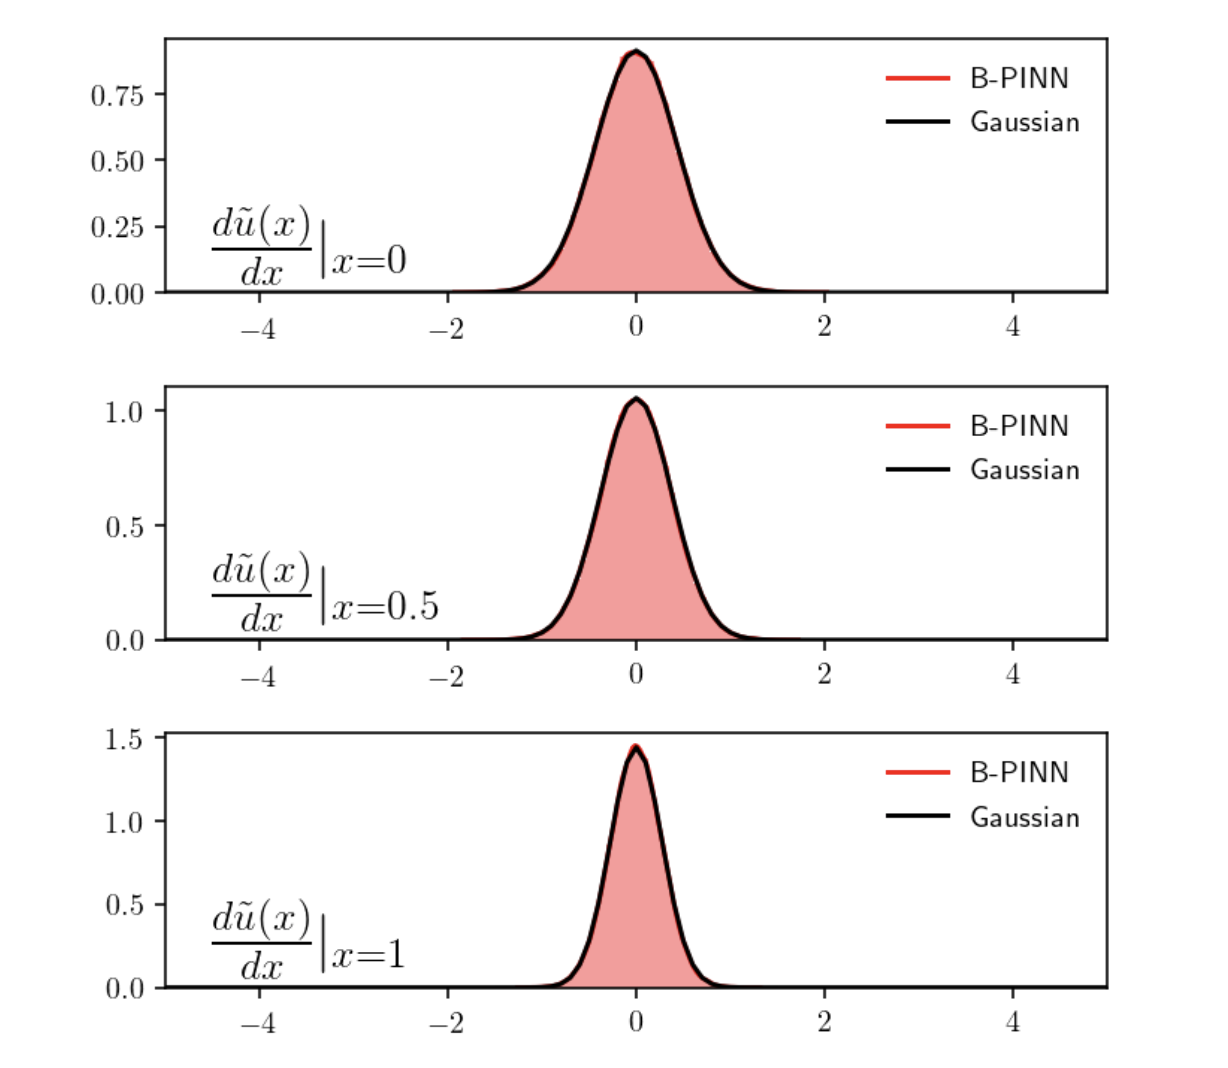
\includegraphics[width=0.6\linewidth]{PINNGP.png}}
  \caption{
 GP of PINN. Three layers with each layer 50 neurons.}
\end{figure}
\end{frame}


\begin{frame}{Neural tangent kernel: definition}
Now, we move onto the optimization step, denote the loss function by $F: \theta \rightarrow \mbR$. The evolution of the function is given by
	\begin{equation*}
\begin{aligned}
	\lp \p_t f\lp x \rp \rp_l = \ & \frac{\p \lp f\lp x \rp \rp_l}{\p \theta} \frac{\p \theta }{\p t}\\
	= & \ \frac{\p \lp f\lp x \rp \rp_l}{\p \theta} \frac{d F\lp \theta \rp }{d \theta}\\
	= & \ \frac{\p \lp f\lp x \rp \rp_l}{\p \theta} \otimes \frac{\p \lp f\lp x \rp \rp_l}{\p \theta} \frac{d F\lp f \rp }{d f}\\
	= & \  \frac{1}{N}\sum_{i = 1}^N\sum_{l' = 1}^{N_L} K_{l', l}\lp x_i, x \rp \lp \frac{d F\lp f \rp }{d f}\lp x_i \rp \rp_{l'}			\\
	= &  \ \frac{1}{N} K\lp x_{D}, x \rp \frac{d F\lp f \rp }{d f}\lp x_{D} \rp
\end{aligned}
\end{equation*}
\end{frame}


\begin{frame}{Neural tangent kernel: convergence}
	We again prove the convergence of NTK by induction. We decompose the set of parameters to two sets: parameters in the outmost layer, parameters remain, i.e.
	\bequn
		\begin{aligned}
		z^{L}\lp \mfx \rp & = \sum_{i = 1}^{N_{L}} W_{i}^{L}y_i^{L}\lp \mfx \rp, 		\\
		\frac{1}{N_{L}}\sum_{i = 1}^{N_{L}}\frac{\p z^{L}\lp \mfx \rp}{\p W_{i}^{L}} \frac{\p z^{L}\lp \mfx' \rp}{\p W_{i}^{L}} & = \frac{1}{N_{L}}\sum_{i = 1}^{N_{L}} y_i^{L}\lp \mfx \rp y_i^{L}\lp \mfx' \rp  = k^L\lp \mfx, \mfx' \rp.
		\end{aligned}
	\eequn
\end{frame}


\begin{frame}{Neural tangent kernel: convergence}
	For the other parameters, we use chain rule, i.e.
	\bequn
		\begin{aligned}
		& \ \frac{1}{N_{L - 1}}\sum_{i = 1}^{N_{L - 1}}\frac{\p z^{L}\lp \mfx \rp}{\p W_{ji}^{L - 1}} \frac{\p z^{L}\lp \mfx' \rp}{\p W_{ji}^{L - 1}} \\
		= & \ \frac{1}{N_{L - 1}}\sum_{i = 1}^{N_{L - 1}}\frac{\p z^{L - 1}\lp \mfx \rp}{\p W_{ji}^{L - 1}} \frac{\p z^{L - 1}\lp \mfx' \rp}{\p W_{ji}^{L - 1}} \phi'\lp z^{L - 1}\lp \mfx \rp \rp \phi'\lp z^{L - 1}\lp \mfx' \rp \rp  \lp W_{j}^L \rp^2 \\
		= & \ \frac{1}{N_L}K^{L - 1}\lp \mfx, \mfx' \rp \mbE_{z \sim \mathcal{GP}\lp \mathbf{0}, k^{L - 1} \rp}\lb \phi'\lp z^{L - 1}\lp \mfx \rp \rp \phi'\lp z^{L - 1}\lp \mfx' \rp \rp \rb.
		\end{aligned}
	\eequn
\end{frame}


\begin{frame}{Neural tangent kernel: convergence}
In the infinite-width limit, the NTK also converges to 
	\begin{figure}[h]
  \centering
  \centerline{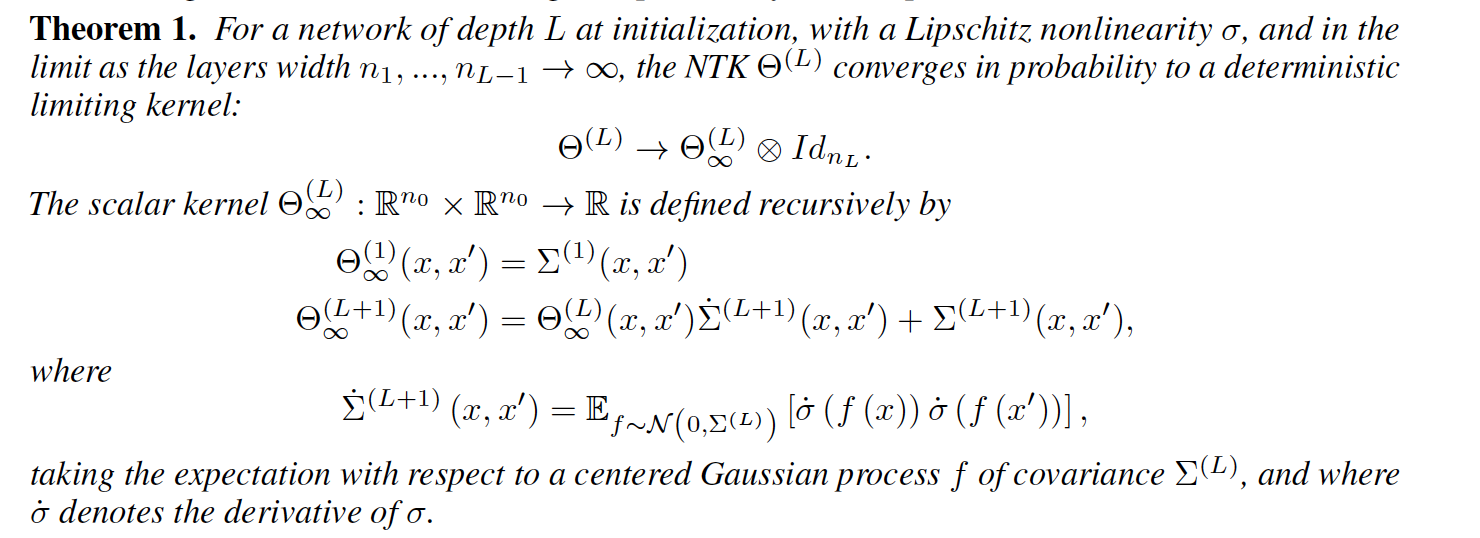
\includegraphics[width=\linewidth]{NTK1.png}}
  \caption{
 Theoretic result on NTK.}
\end{figure}
\footnotetext{Arthur Jacot, Franck Gabriel, and Clement Hongler. Neural tangent kernel: Convergence and general- ization in neural networks, 2018.}
\end{frame}


\begin{frame}{GP for PINN: Three layer NN}
	\begin{figure}[h]
  \centering
  \centerline{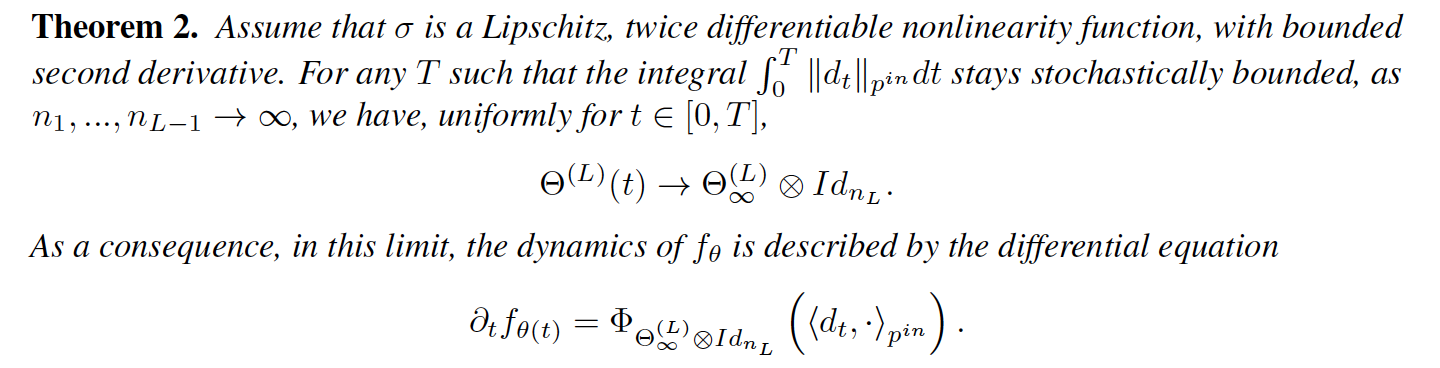
\includegraphics[width=\linewidth]{NTK2.png}}
  \caption{
 Theoretic result on NTK.}
\end{figure}
\begin{figure}[h]
  \centering
  \centerline{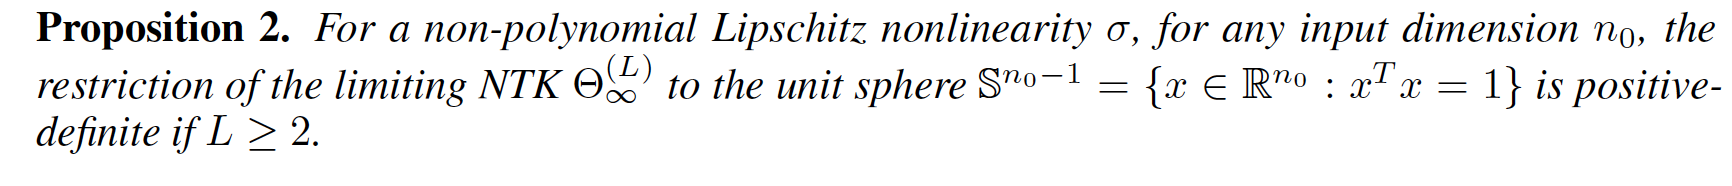
\includegraphics[width=\linewidth]{NTK3.png}}
  \caption{
 Positivity of NTK.}
\end{figure}
\footnotetext{Arthur Jacot, Franck Gabriel, and Clement Hongler. Neural tangent kernel: Convergence and general- ization in neural networks, 2018.}
\end{frame}


\begin{frame}{Comparison of NNGP and NT kernel}
	In linear model where one does not apply non-linearity to the input, it is easy to conclude that two kernels coincide. While in general, they differ from each other in the sense that NNGP kernel describes the behavior of neural network under Bayesian computation, i.e. calculate the Bayesian posterior and NTK describes that under the setting of gradient descent dynamics. Moreover, computing the Bayesian posterior is equivalent to gradient descent with all but the last-layer weights frozen.
\end{frame}


\begin{frame}{Infinite-width neural network as GP: inference}
Viewing infinite-width neural network as GP, we can do GP regression using this GP kernel. Given data $x_D, y_D$, we want to estimate a function s.t. $f\lp x_D \rp = y_D$ and calculate its value at some points $x$.		\\
\indent
Noisy case:
\bequn
\begin{aligned}
    \mu_b(x) &= k(x, x_D)(k(x_D, x_D) + \sigma^2 I)^{-1}y_D\\
    k_b(x, x') &= k(x, x') - k(x, x_D) (k(x_D, x_D) + \sigma^2 I)^{-1} k(x_D, x')
\end{aligned}
\eequn
\indent
Unnoisy case:
\bequn
\begin{aligned}
    \mu_b(x) &= k(x, x_D)k(x_D, x_D)^{-1}y_D\\
    k_b(x, x') &= k(x, x') - k(x, x_D) k(x_D, x_D) ^{-1} k(x_D, x')
\end{aligned}
\eequn
\end{frame}


\begin{frame}{Infinite-width neural network training as kernel gradient flow}
\begin{equation*}
    \partial_t f(x) \frac{1}{N} K\lp x_{D}, x \rp \frac{d F\lp f \rp }{d f}\lp x_{D} \rp, \partial_t f(x_D) = \frac{1}{N}K(x_D, x_D) d|_{f_t}(x_D),
\end{equation*}
\begin{equation*}
    \partial_tf(x) = K(x, x_D)K^{-1}(x_D, x_D) \partial_tf(x_D)
\end{equation*}
Consequently, we have the following characteristic for training trajectory.
	\begin{equation}\label{eqn:finfity}
\begin{aligned}
f_\infty(x) &= f_0(x) + \int_0^\infty \partial_tf(x)dt \\
            &= f_0(x) + K(x, x_D)K^{-1}(x_D, x_D)  \int_0^\infty \partial_tf(x_D) dt \\
            &= f_0(x) + K(x, x_D)K^{-1}(x_D, x_D) (f_\infty(x_D) - f_0(x_D)) \\
            &= K(x, x_D)K^{-1}(x_D, x_D) f_\infty(x_D) + \\
            & \quad \left[f_0(x) - K(x, x_D)K^{-1}(x_D, x_D) f_0(x_D)\right]\\
\end{aligned}
\end{equation}
\end{frame}


\begin{frame}{Neural network training as kernel gradient flow}
	We can further calculate the mean and variance for the neural tangent kernel.
	\begin{equation*}\label{eqn:ensembleinfty}
\begin{aligned}
    \mu_e(x) &= K(x, x_D)K(x_D, x_D)^{-1}y_D\\
    K_e(x, x') &= k(x, x') - K(x, x_D)K(x_D, x_D)^{-1} k(x_D, x') \\
    & -  K(x', x_D) K(x_D, x_D)^{-1} k(x_D, x) \\
    & + K(x, x_D) K(x_D, x_D)^{-1}k(x_D,x_D) K(x_D, x_D)^{-1}K(x_D,x'),
\end{aligned}
\end{equation*}
This coincides with the Bayesian posterior for NNGP kernel if we have $k = K$. NNGP regression can be viewed as training only the last layer.
\end{frame}


\begin{frame}{Numerical experiment of GPK and NTK: initialization}
	\begin{figure}[H]
  \centering
  \centerline{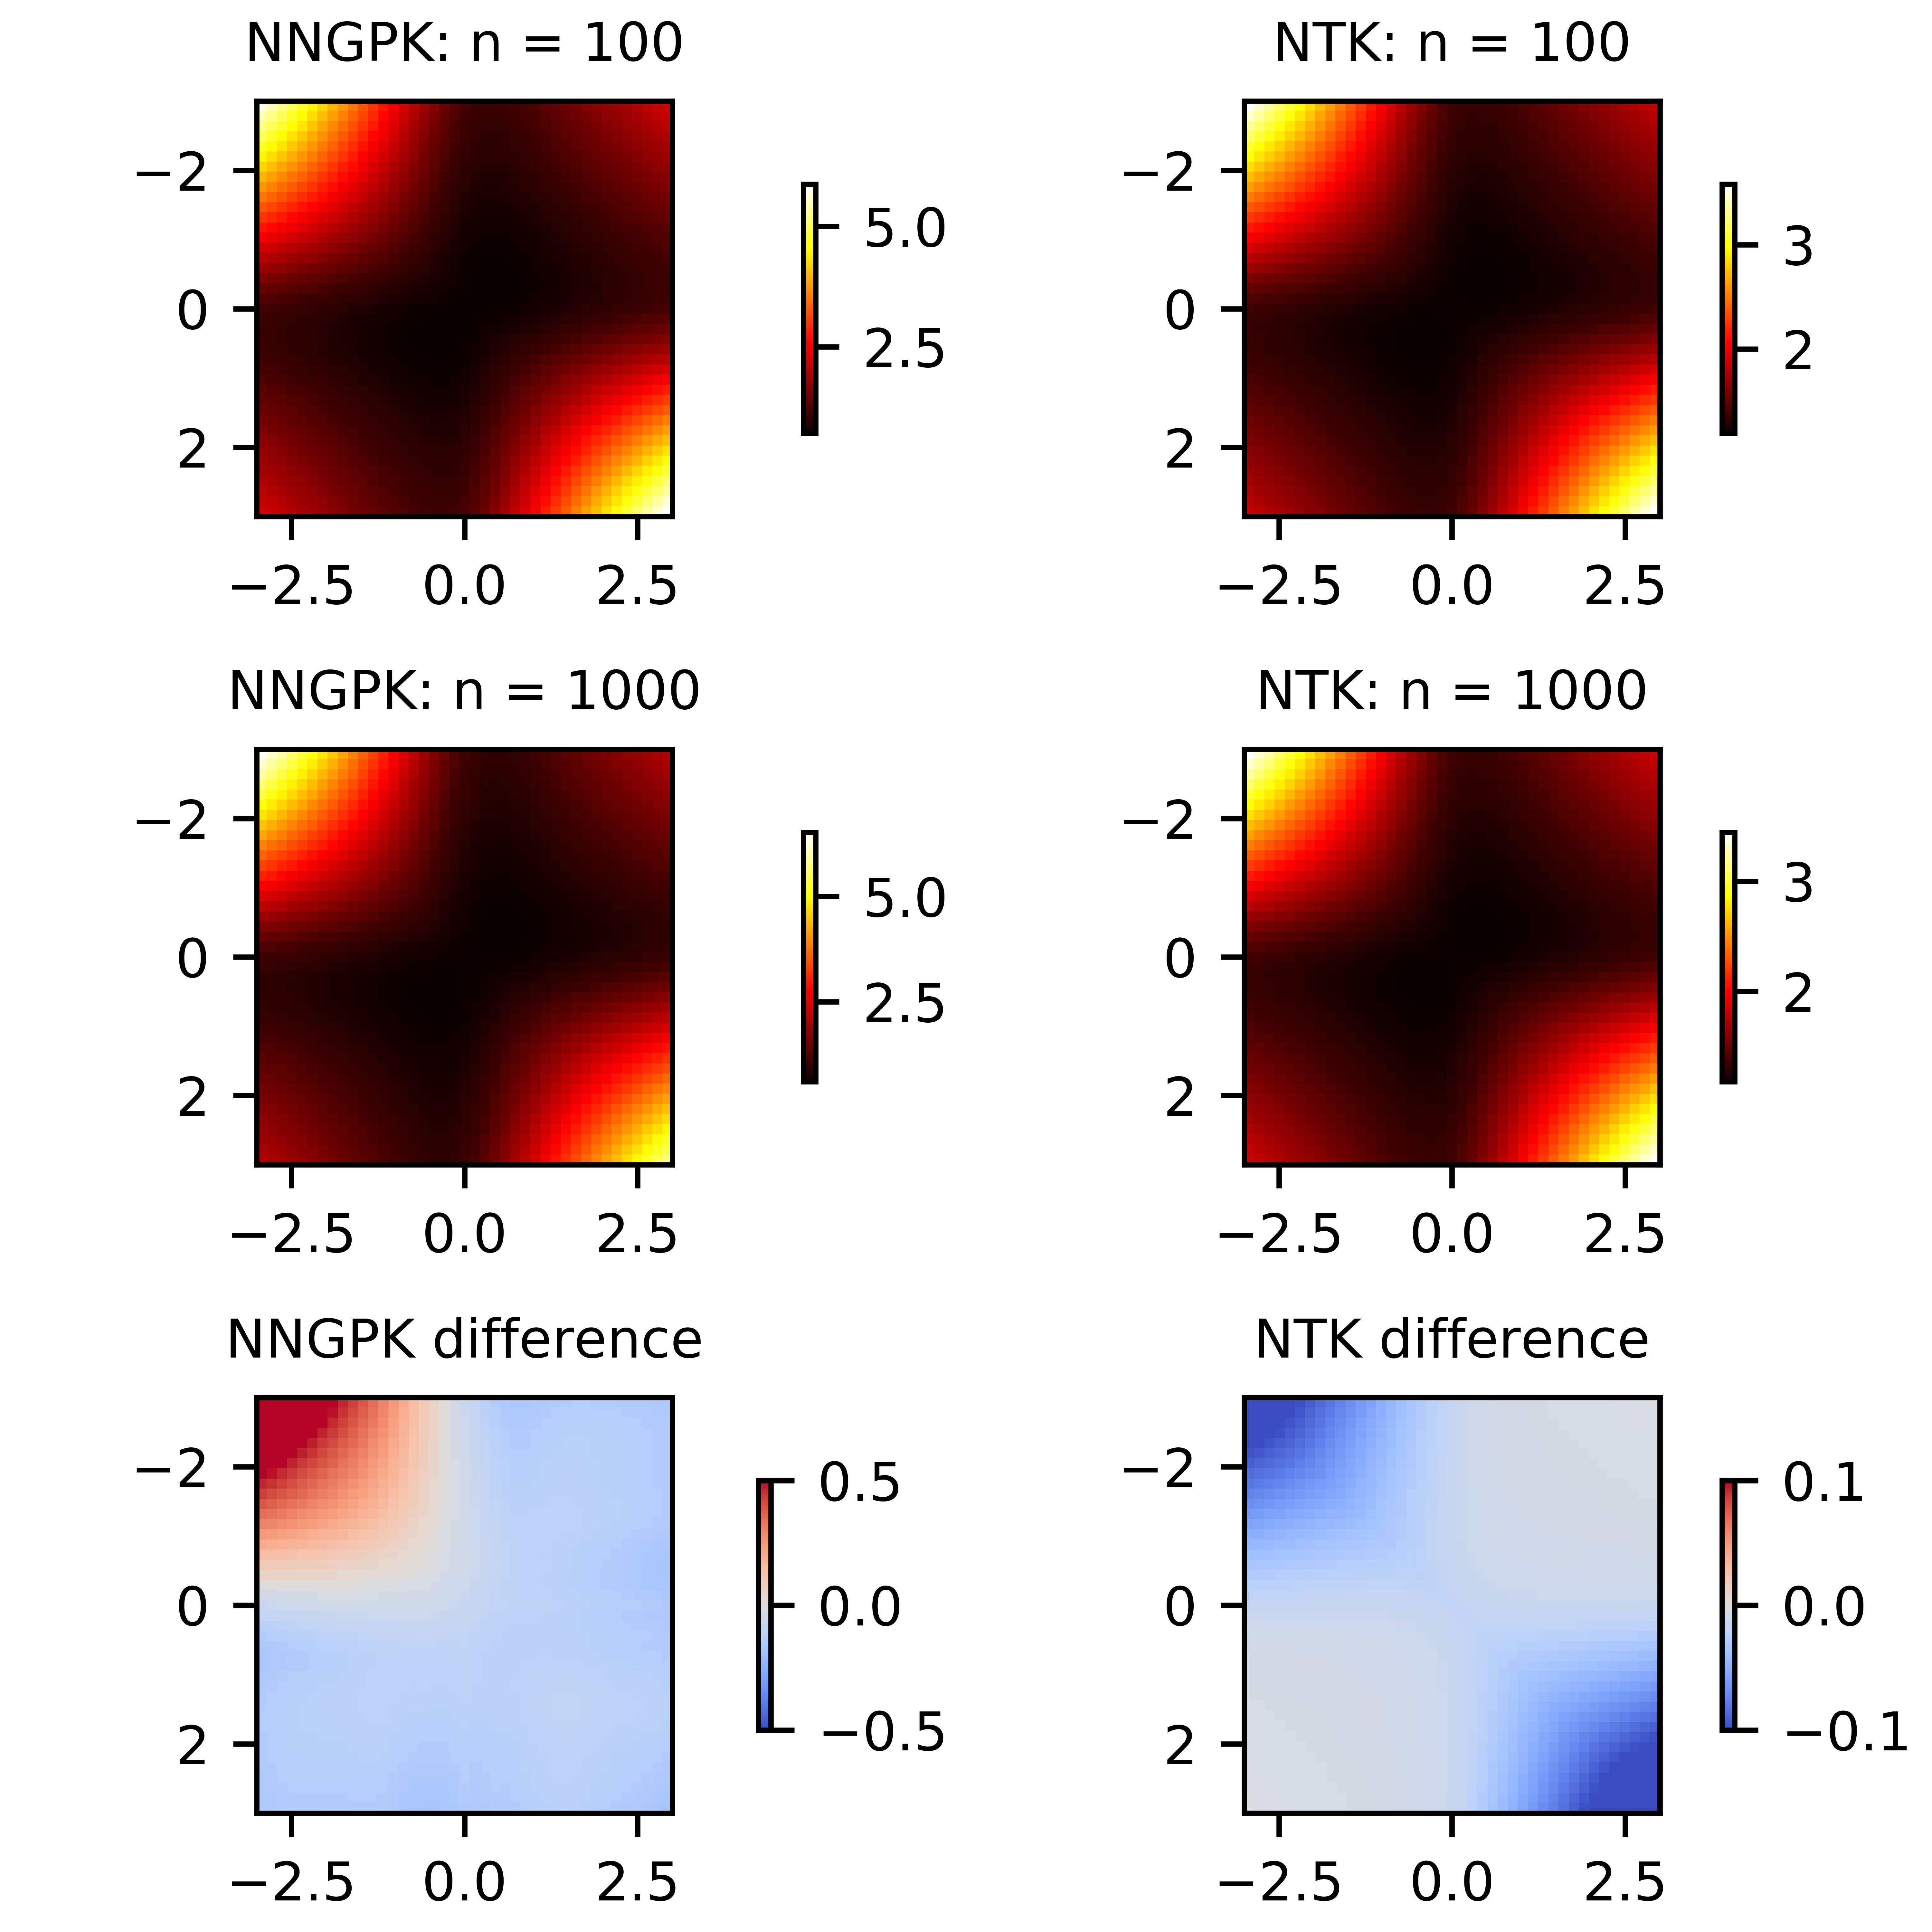
\includegraphics[width=0.6\linewidth]{kernel-init.jpg}}
  \caption{
  First row, 2000 samples of a network with $L = 2, N_1 = N_2 = 100$ and a sigmoid linearity. Second row, 200 samples with $N_1 = N_2 = 1000$.}
\end{figure}
\end{frame}


\begin{frame}{Numerical experiment of GPK and NTK: Over-parametrized training}
	\begin{figure}[h]
  \centering
  \centerline{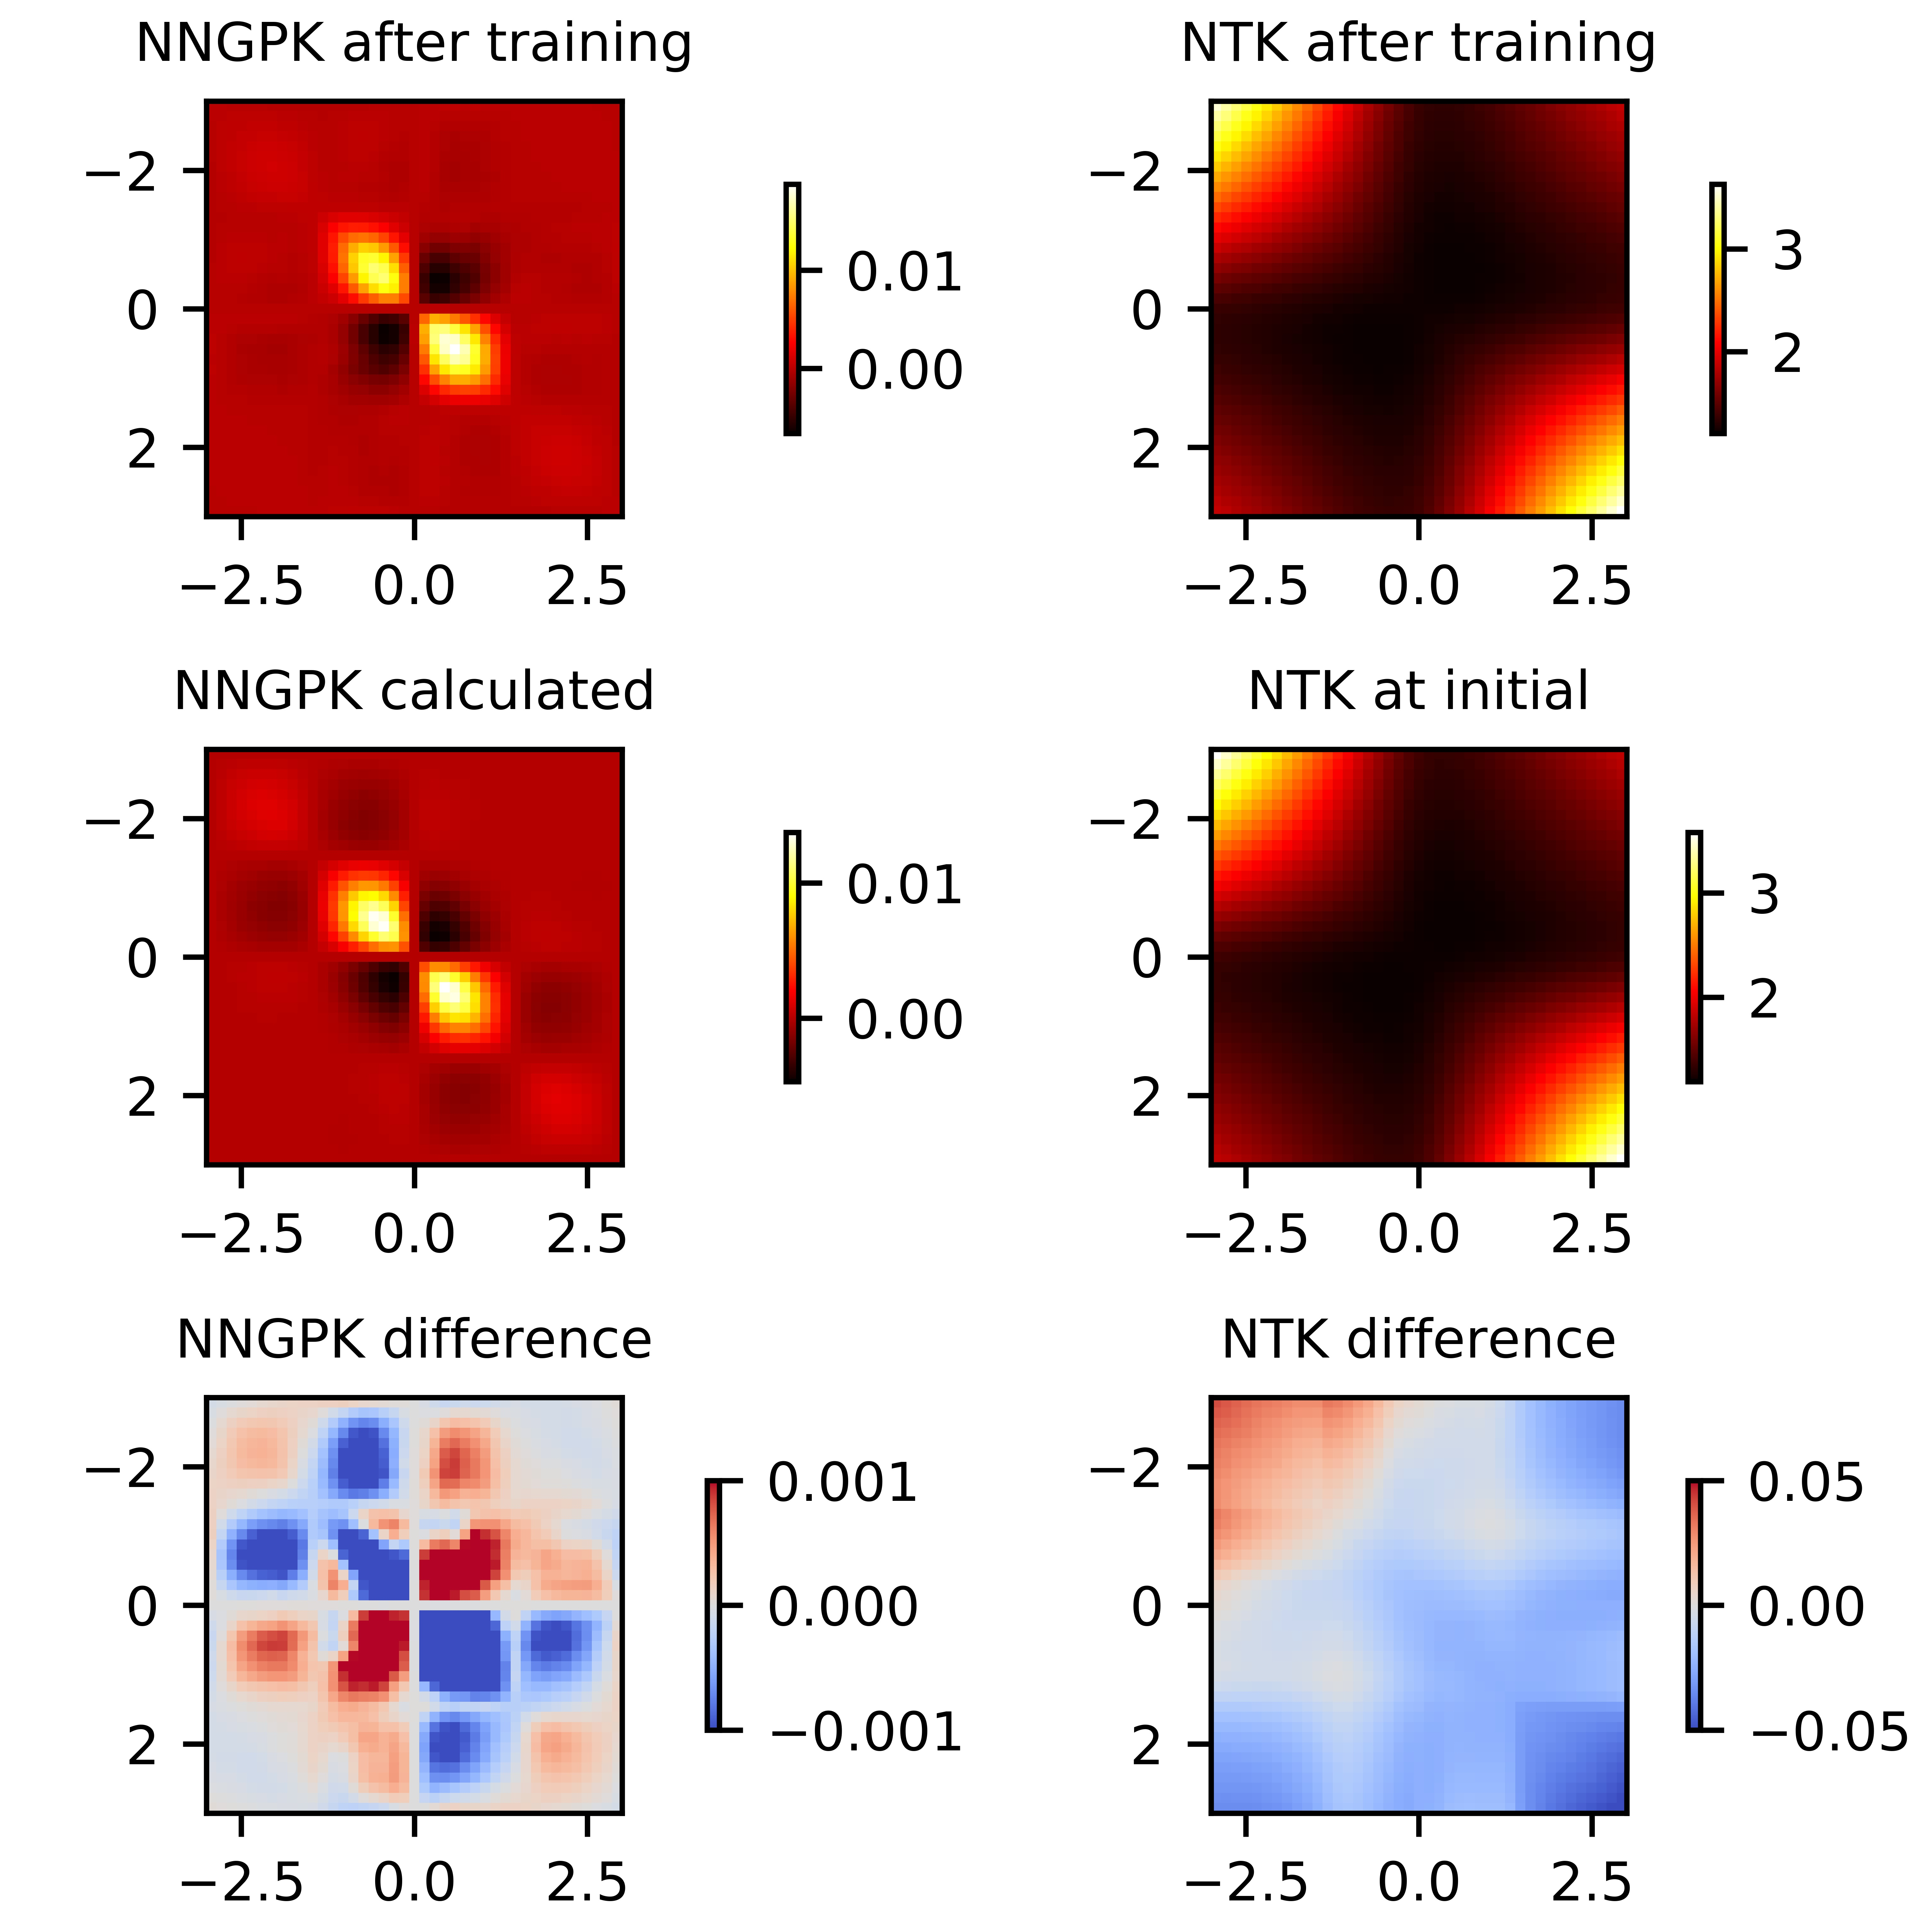
\includegraphics[width=0.6\linewidth]{kernel-train.jpg}}
  \caption{
  2000 samples of a network with $L = 2, N_1 = N_2 = 30$ and a sigmoid linearity, training for 200 epochs on 5 data points.}
\end{figure}
\end{frame}


\begin{frame}{Numerical experiment of GPK and NTK: Not over-parametrized training}
	\begin{figure}[h]
  \centering
  \centerline{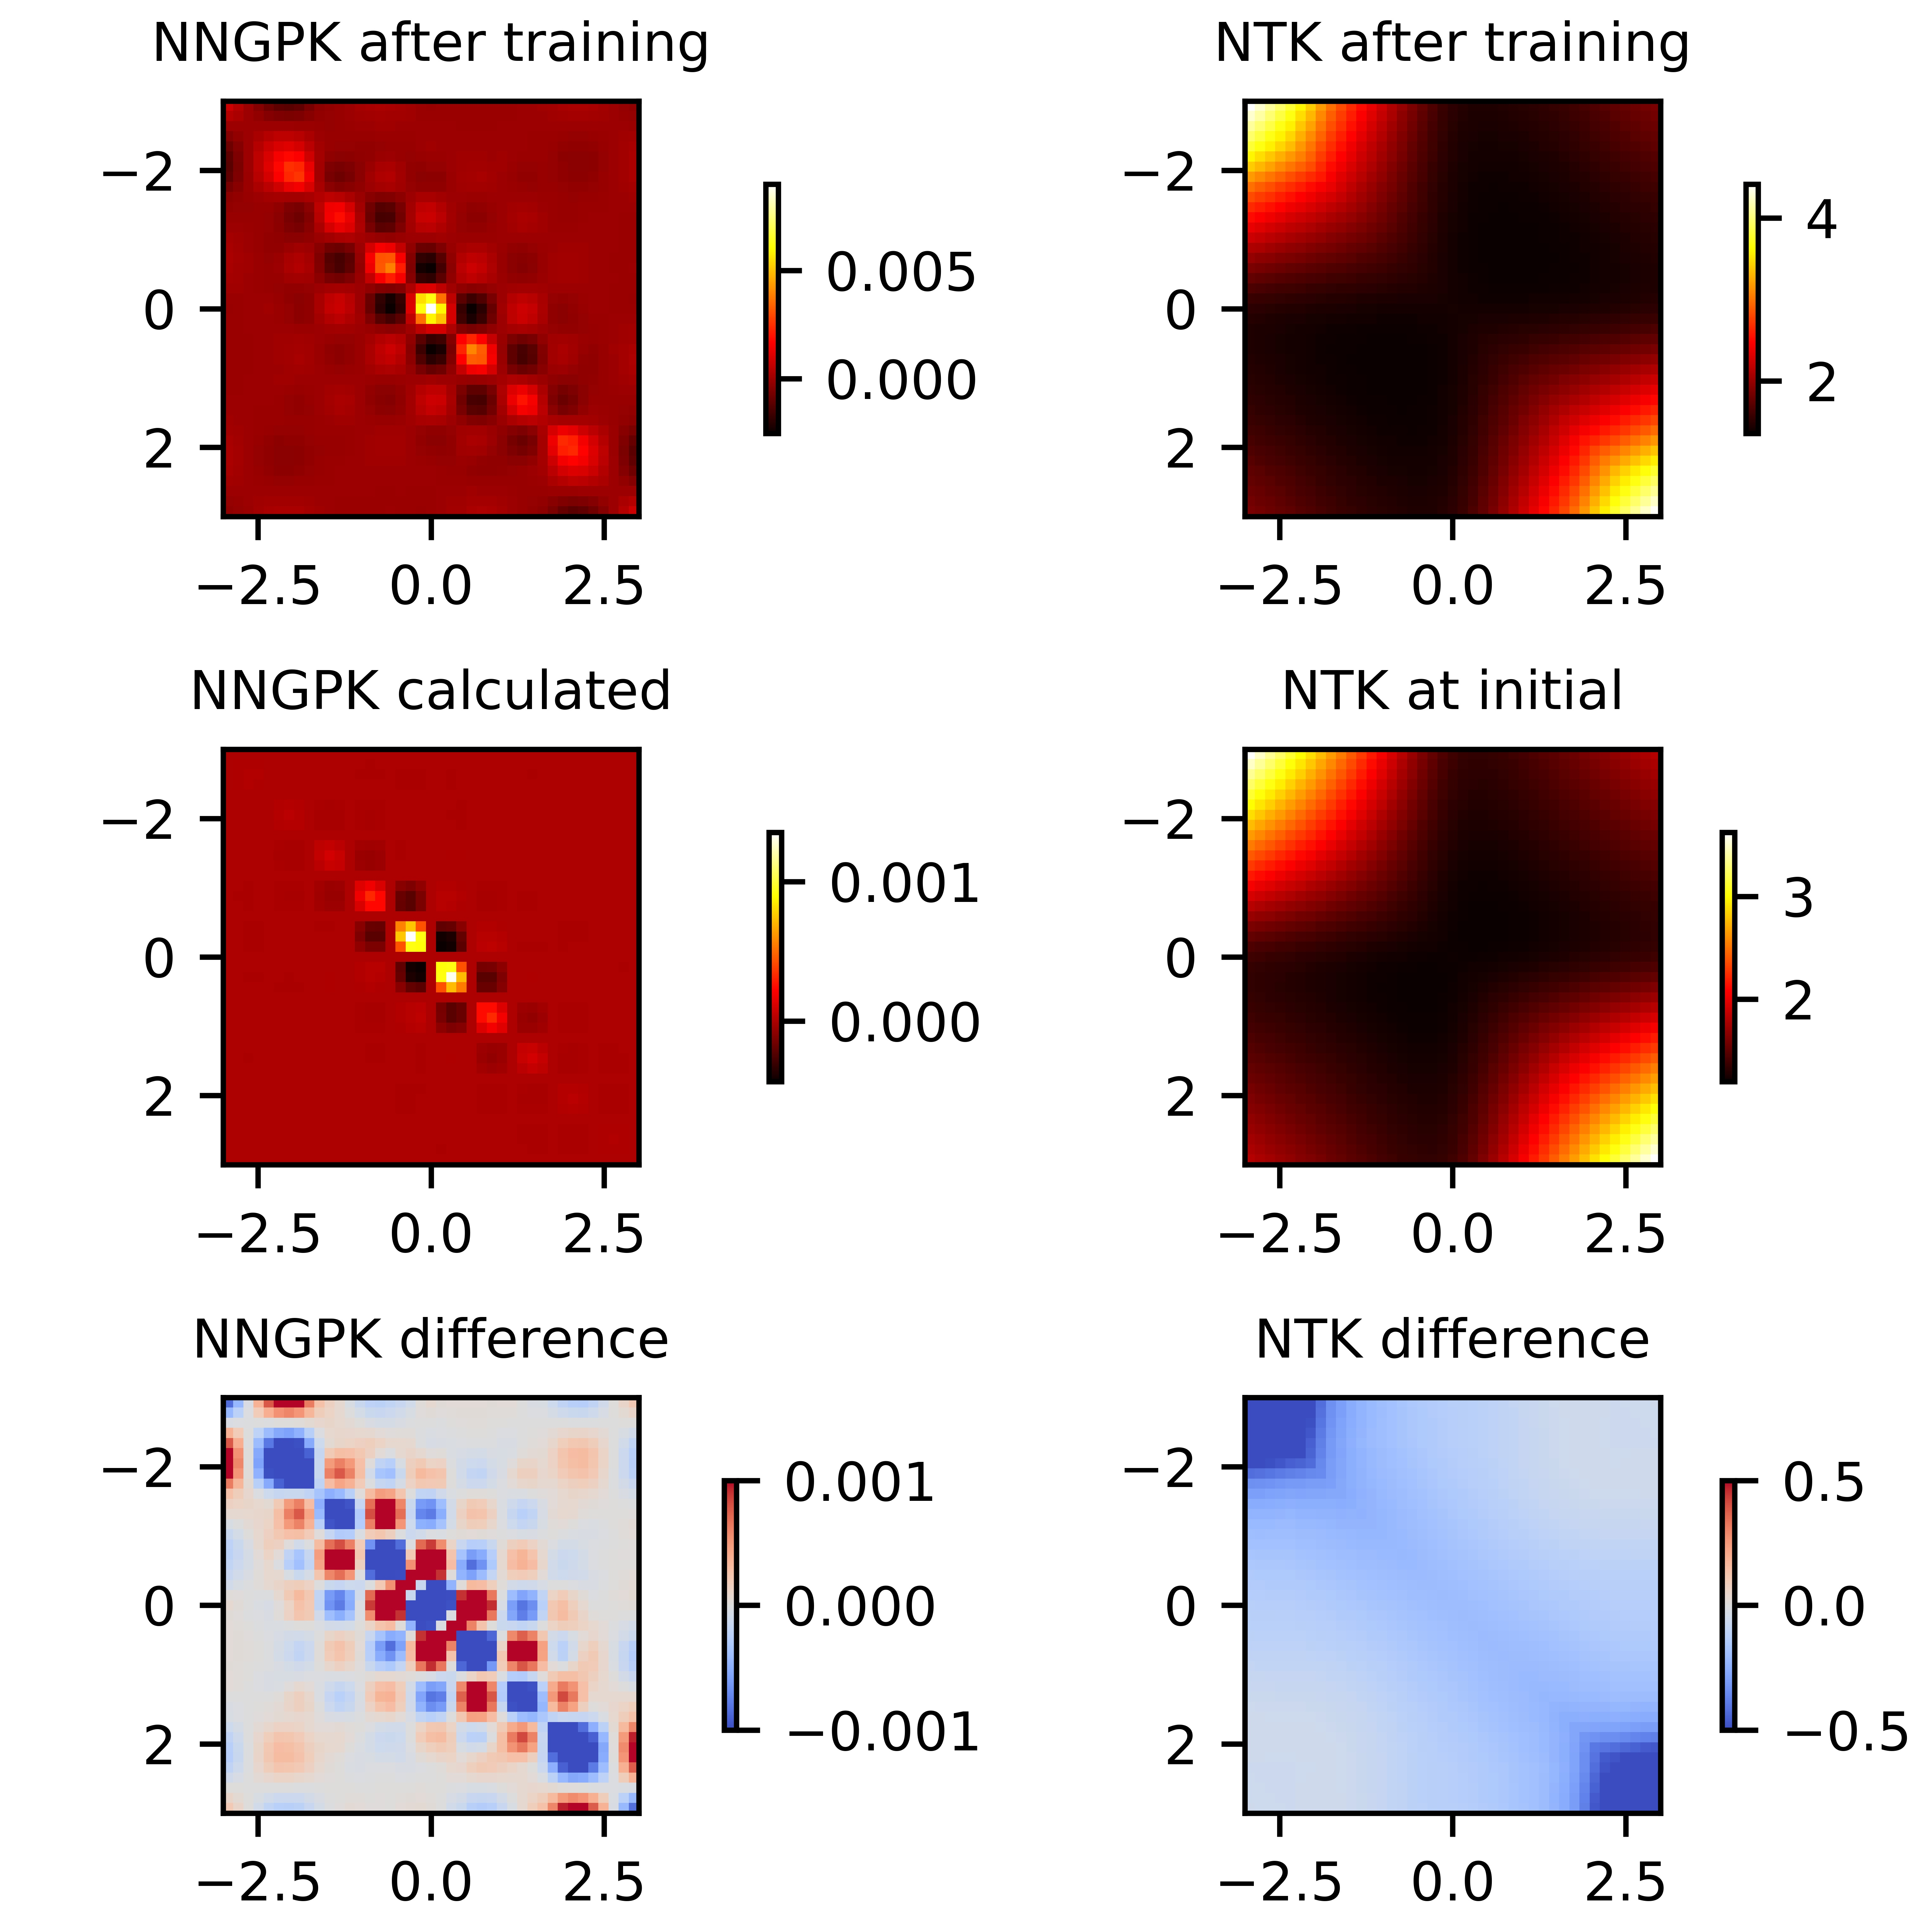
\includegraphics[width=0.6\linewidth]{kernel-train-notover.jpg}}
  \caption{
  2000 samples of a network with $L = 2, N_1 = N_2 = 30$ and a sigmoid linearity, training for 200 epochs on 10 data points.}
\end{figure}
\end{frame}


\begin{comment}
\begin{frame}{Generalized arcsine law: double Laplace transform formula}
	\begin{equation}\label{double-laoplace}
	\begin{aligned}
    & \ \int_0^{\infty} e^{-\mu t} \mbE\lb \exp\lbb -\sum_{i = 1}^N \lambda_i A_i\lp t \rp \rbb \rb dt \\
    = & \ \frac{1}{\sum_{i = 1}^N \psi\lp \lambda_i + \mu \rp}\lp \sum_{i = 1}^N \frac{\psi\lp \lambda_i + \mu \rp}{\lambda_i + \mu} \rpz.
    \end{aligned}
\end{equation}
\end{frame}
\end{comment}


\begin{frame}{Comparison between NNGP regression and neural network training}
	How does this NNGP regression relates to the network training using gradient descent, here is some experiments.	\begin{figure}[h]
  \centering
  \centerline{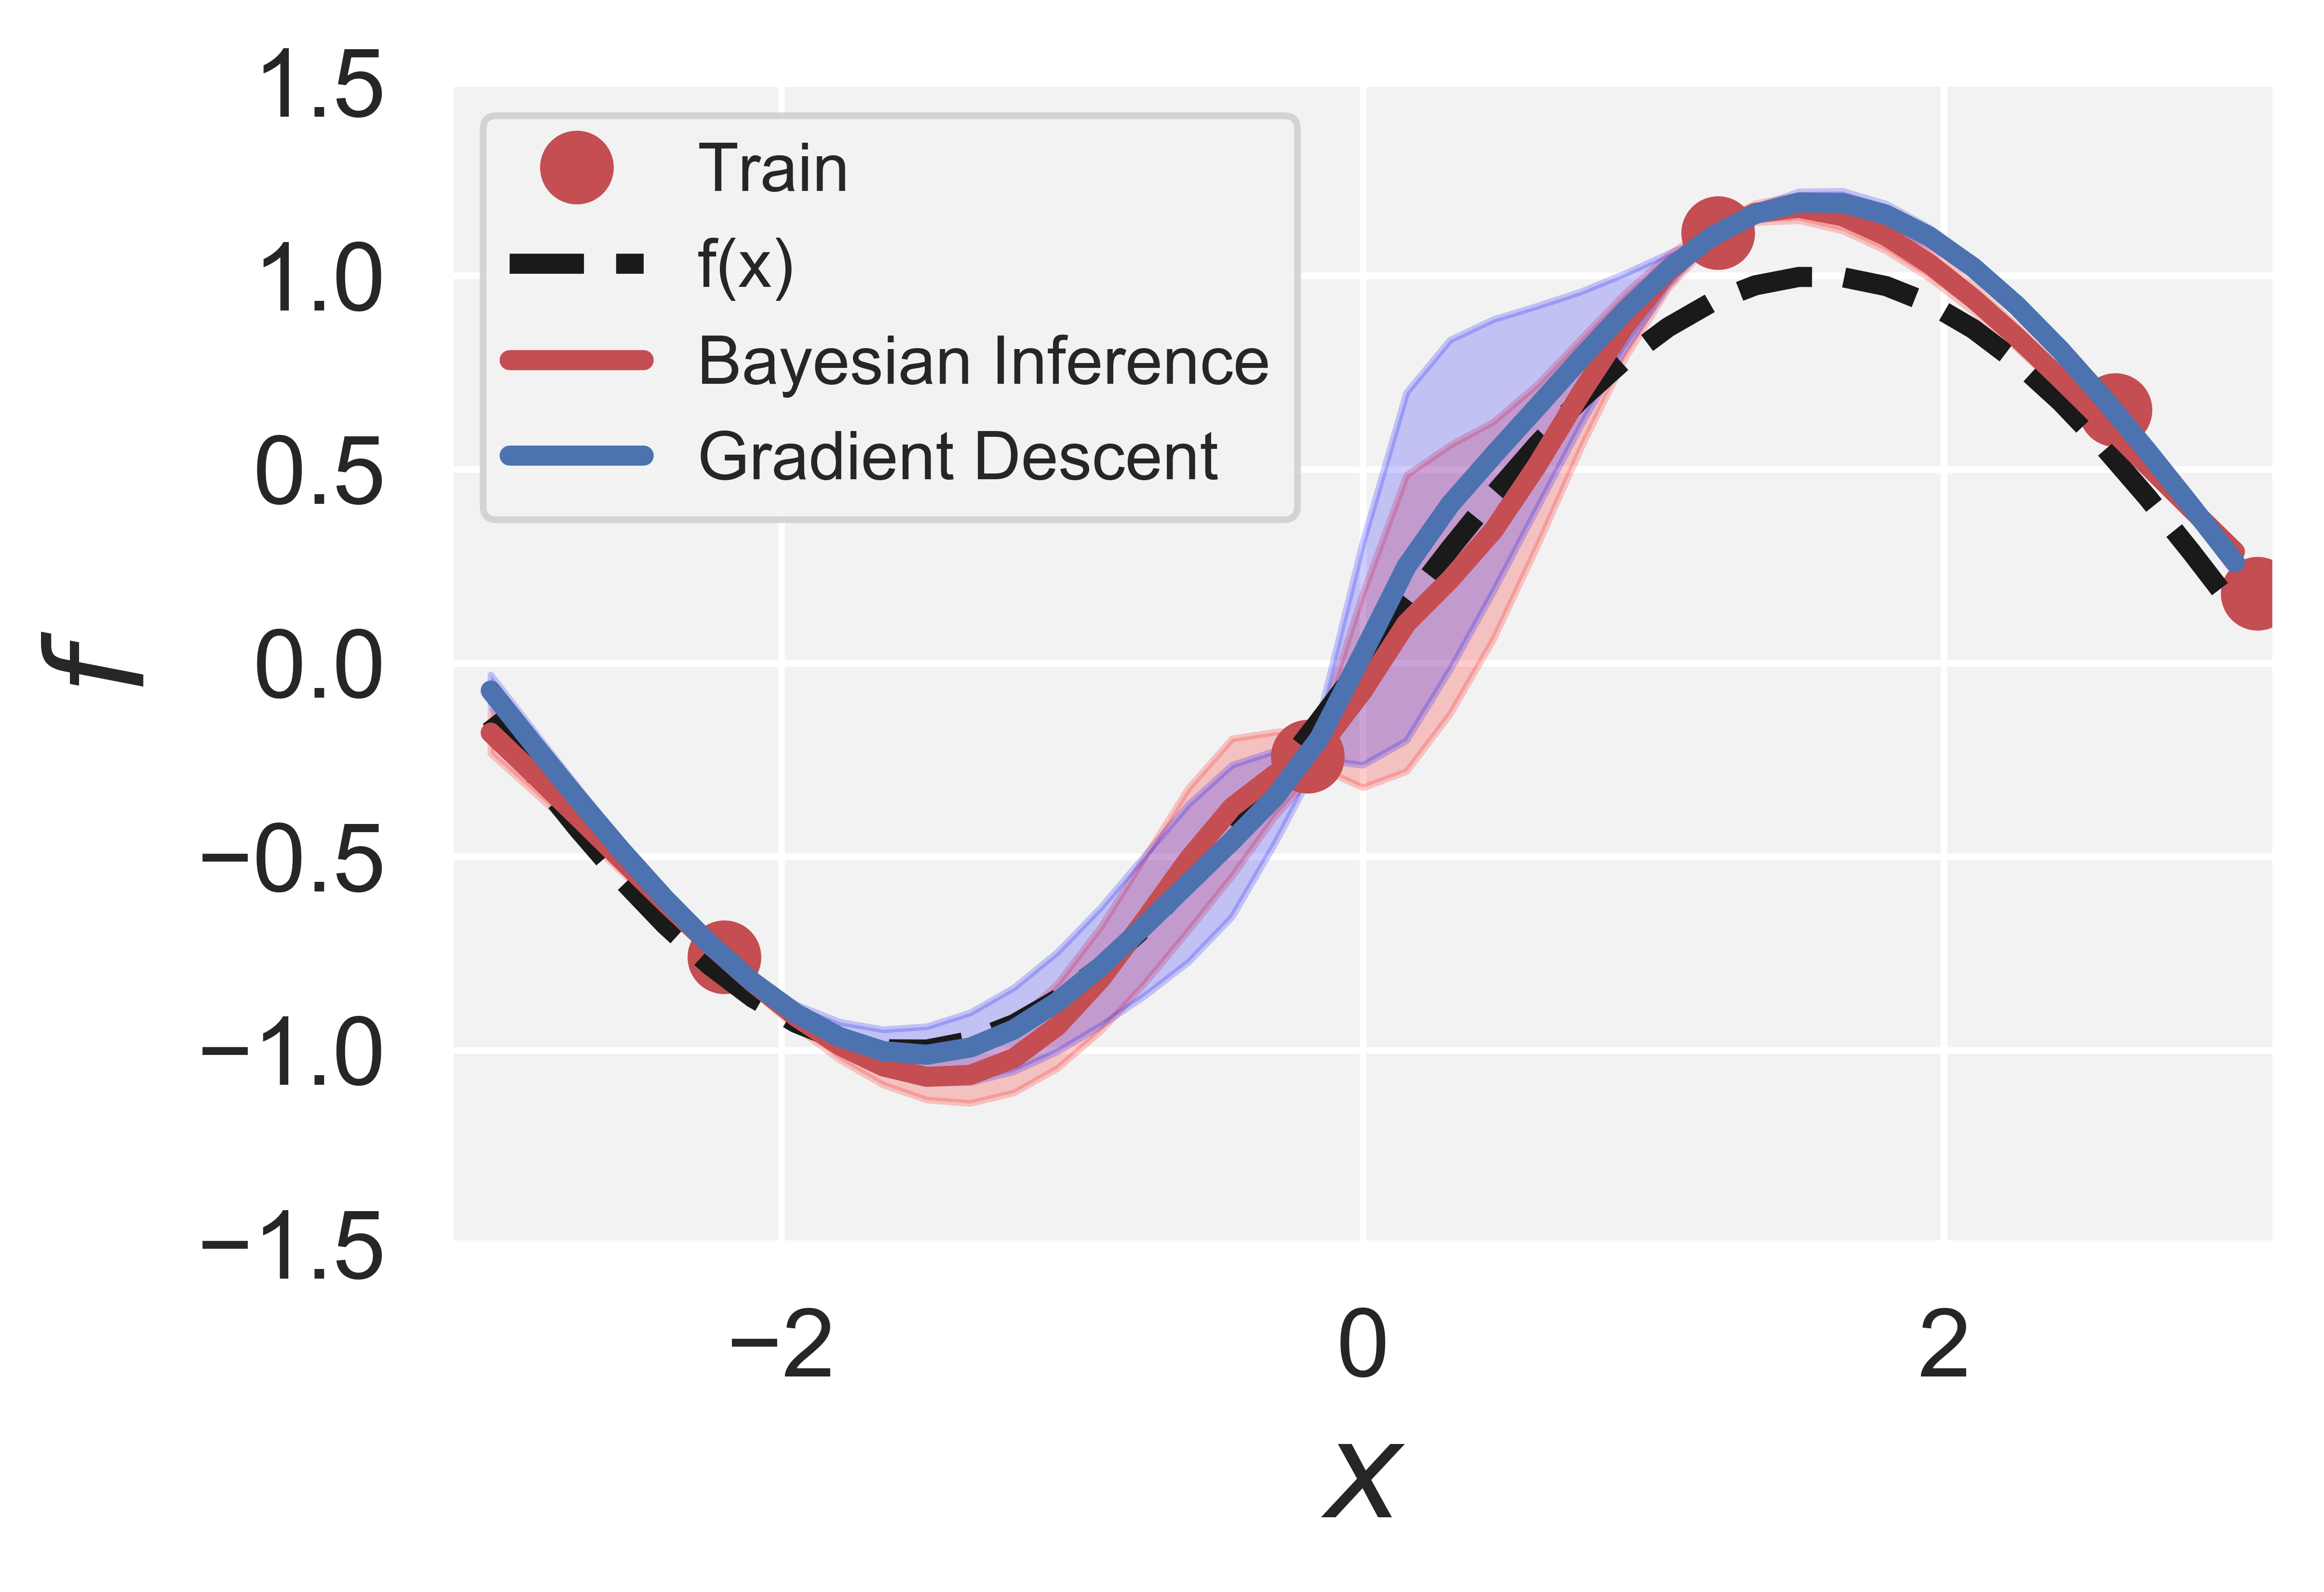
\includegraphics[width=0.6\linewidth]{comp.png}}
  \caption{
  A comparison between NNGP and NTK. }
\end{figure}
\end{frame}


\begin{frame}{NNGP for NAS}
	What are the advantages of NNGP regression comparing to training of NN? 
	\begin{itemize}
		\item NNGP regression is more efficient, especially when the number of samples is small.
		\item The result of NNGP regression is correlated to network’s actual performance after training, as illustrated in the infinite width.
	\end{itemize}
\end{frame}


\begin{frame}
	Thanks for listening.
\end{frame}


\begin{comment}
\begin{frame}{Generalized arcsine law: $t_{\max}$ of stochastic processes}
The distribution of $t_{\max}$ of the following stochastic processes is calculated by the methods of path-integral\footnote{S. N. Majumdar and J.-P. Bouchaud. Optimal time to sell a stock in the Black-Scholes model: comment on 'Thou shalt buy and hold', by Shiryaev, Z. Xu and X. Y. Zhou. Quant.\ Finance 8, 753 (2008).}\textsuperscript{,}\footnote{S. N. Majumdar, J. Randon-Furling, M. J. Kearney and M. Yor. On the time to reach maximum for a variety of constrained Brownian motions. J. Phys.\ A 41, 365005 (2008).}, agreement formulae\textsuperscript{7} and renormalization group\footnote{G. Schehr and P. Le Doussal. Extreme value statistics from the real space renormalization group: Brownian motion, Bessel processes and continuous time random walks. J. Stat.\ Mech.\ (2010) P01009.}.
\begin{itemize}
	\item 1. Brownian bridge, reflected Brownian bridge, Brownian excursion, Brownian meander, Brownian motion with drift, Bessel process, Bessel bridge.
	\item 2. Discrete-time random walk.
	\item 3. Run-and-tumble particle.
\end{itemize}
\end{frame}


\begin{frame}{Generalized arcsine law: $t_{\max}$ of Brownian bridge and reflected Brownian bridge}
Denote $X_t^\text{bri}$ as a Brownian bridge on $[0,T]$, which is defined as a Brownian motion, $X_t$, constrained such that $X_0 = 0$ and $X_T = 0$. Define $X_t^\text{ref bri} := \left|X_t^\text{bri}\right|$ which denotes a reflected Brownian bridge on $[0,T]$. The time of the maximum is denoted by:
\begin{equation}
    \begin{aligned}
        t_\text{max}^\text{bri} & := \frac{1}{T}\arg \max_{t \in [0, T]} X_t^\text{bri},  \\
        t_\text{max}^\text{ref bri} & := \frac{1}{T}\arg \max_{t \in [0, T]} X_t^\text{ref bri}.
    \end{aligned}
\end{equation}
\end{frame}

\begin{frame}{Generalized arcsine law: $t_{\max}$ of Brownian bridge and reflected Brownian bridge}
\begin{Thm}[Distribution of $t_{\max}$ of Brownian bridge\footnotemark, 1957]
$t_\text{max}^\text{bri}$ obeys uniform distribution
:
\begin{equation}
    p(x) = 1, \quad x \in [0, 1].
\end{equation}
\end{Thm}
\footnotetext{W. Feller. An introduction to probability theory and its applications. John Wiley and Sons, Inc.\ 1957.}
\end{frame}

\begin{frame}{Generalized arcsine law: $t_{\max}$ of Brownian bridge and reflected Brownian bridge}
\begin{Thm}[Distribution of $t_{\max}$ of reflected Brownian bridge\footnotemark, 2008]
$t_\text{max}^\text{ref bri}$ obeys the law as follows:
\begin{multline}
    p(x) = 2\sum_{n,m=0}^\infty (-1)^{m+n} \frac{(2m+1)(2n+1)}{\left[(2n+1)^2x+(2m+1)^2(1-x)\right]^{3/2}}, \\
    x \in [0, 1].
\end{multline}
\end{Thm}
\footnotetext{S. N. Majumdar, J. Randon-Furling, M. J. Kearney and M. Yor. On the time to reach maximum for a variety of constrained Brownian motions. J. Phys.\ A 41, 365005 (2008).}
\end{frame}

\begin{frame}{Generalized arcsine law: $t_{\max}$ of Brownian excursion and Brownian meander}
Denote $X_t^\text{ex}$ as a Brownian excursion on $[0,T]$, which is defined as a Brownian motion, $X_t$, constrained so that $X_0 = 0, X_T = 0$ with $X_t > 0$ for $t \in (0,T)$. Denote $X_t^\text{mea}$ as a Brownian meander on $[0,T]$, which is defined as a Brownian motion, $X_t$, constrained so that $X_0 = 0$ with $X_t > 0$ for $t \in (0,T]$. The time of the maximum is denoted by:
\begin{equation}
    \begin{aligned}
        t_\text{max}^\text{ex} & := \frac{1}{T}\arg \max_{t \in [0, T]} X_t^\text{ex},  \\
        t_\text{max}^\text{mea} & := \frac{1}{T}\arg \max_{t \in [0, T]} X_t^\text{mea}.
    \end{aligned}
\end{equation}
\end{frame}

\begin{frame}{Generalized arcsine law: $t_{\max}$ of Brownian excursion and Brownian meander}
\begin{Thm}[Distribution of $t_{\max}$ of Brownian excursion\footnotemark, 2008]
$t_\text{max}^\text{ex}$ obeys the law as follows:
\begin{equation}
    p(x) = 3\sum_{n,m=1}^\infty (-1)^{m+n} \frac{m^2n^2}{\left[n^2x+m^2(1-x)\right]^{5/2}}, \quad x \in [0, 1].
\end{equation}
\end{Thm}
\footnotetext{S. N. Majumdar, J. Randon-Furling, M. J. Kearney and M. Yor. On the time to reach maximum for a variety of constrained Brownian motions. J. Phys.\ A 41, 365005 (2008).}
\end{frame}

\begin{frame}{Generalized arcsine law: $t_{\max}$ of Brownian excursion and Brownian meander}
\begin{Thm}[Distribution of $t_{\max}$ of Brownian meander\footnotemark, 2008]
$t_\text{max}^\text{mea}$ obeys the law as follows:
\begin{equation}
    p(x) = 2\sum_{m=0,n=1}^\infty (-1)^{n+1} \frac{n^2}{\left[n^2x+(2m+1)^2(1-x)\right]^{3/2}}, x \in [0, 1].
\end{equation}
\end{Thm}
\footnotetext{S. N. Majumdar, J. Randon-Furling, M. J. Kearney and M. Yor. On the time to reach maximum for a variety of constrained Brownian motions. J. Phys.\ A 41, 365005 (2008).}
\end{frame}

\begin{frame}{Generalized arcsine law: $t_{\max}$ of Brownian motion with drift}
Define $X_t^{(\mu)} := X_t+\mu t$ which denotes a Brownian motion with drift on $\mbR$. The time of the maximum within the period $[0,T]$ is denoted by:
\begin{equation}
    t_\text{max}^{(\mu)} := \frac{1}{T}\arg \max_{t \in [0, T]} X_t^{(\mu)}.
\end{equation}
\end{frame}

\begin{frame}{Generalized arcsine law: $t_{\max}$ of Brownian motion with drift}
\begin{Thm}[Distribution of $t_{\max}$ of Brownian motion with drift\footnotemark, 2003]
$t_\text{max}^{(\mu)}$ obeys the law as follows:
\begin{multline}
    p(x;\Tilde{\mu}) = 2 \left[\frac{\varphi \left(\Tilde{\mu}\sqrt{x}\right)}{\sqrt{x}} + \Tilde{\mu}\Phi\left(\Tilde{\mu}\sqrt{x}\right)\right] \times \\
    \left[\frac{\varphi \left(\Tilde{\mu}\sqrt{1-x}\right)}{\sqrt{1-x}} - \Tilde{\mu}\Phi\left(-\Tilde{\mu}\sqrt{1-x}\right)\right], x \in [0, 1],
\end{multline}
where $\Tilde{\mu} = \mu \sqrt{T}$ and $\varphi (y) = \frac{1}{\sqrt{2\pi}}e^{-y^2/2}$, $\Phi (z) = \int_{-\infty}^z \varphi (y) \, \mathrm{d} y$ denote the standard Gaussian density and distribution function respectively.
\end{Thm}
\footnotetext{E. Buffet. On the time of the maximum of Brownian motion with drift. J. Appl.\ Math.\ Stoch.\ Anal.\ 16, 201 (2003).}
\end{frame}

\begin{frame}{Generalized arcsine law: $t_{\max}$ of Bessel process and Bessel bridge}
Denote $X_t^\text{Bes}$ as a Bessel process on $\mbR$, i.e.\ the radius of the $d$-dimensional Brownian motion $X_t^\text{Bes} = \sqrt{\sum_{i=1}^d (X_t^i)^2} + X_0^\text{Bes}$, where $X_t^1,X_t^2,\dots ,X_t^d$ are $d$ independent Brownian motion, $X_0^\text{Bes} \geqslant 0$. Denote $X_t^\text{Bes bri}$ as a Bessel bridge on $[0,T]$, which is defined as a Bessel process, $X_t^\text{Bes}$, constrained such that $X_0^\text{Bes} = 0$ and $X_T^\text{Bes} = 0$. Define the random variables as follows:
\begin{equation}
\begin{aligned}
    X_\text{max}^\text{Bes} & := \max_{t \in [0, T]} X_t^\text{Bes}, \\
    t_\text{max}^\text{Bes} & := \frac{1}{T}\arg \max_{t \in [0, T]} X_t^\text{Bes}, \\
    t_\text{max}^\text{Bes bri} & := \frac{1}{T}\arg \max_{t \in [0, T]} X_t^\text{Bes bri}.
\end{aligned}
\end{equation}
\end{frame}

\begin{frame}{Generalized arcsine law: $t_{\max}$ of Bessel process and Bessel bridge}
\begin{Thm}[Distribution of $t_{\max}$ of Bessel process\footnotemark, 2010]
$\left(t_\text{max}^\text{Bes}, X_\text{max}^\text{Bes}, X_T^\text{Bes}\right)$ obeys the law as follows:
\begin{multline}
    p(x,u,u_T;u_0,\nu) = \frac{4}{u^5} \frac{u_T^{\nu+1}}{u_0^\nu} \sum_{n,m=1}^\infty j_{\nu,n}j_{\nu,m} \frac{J_\nu (j_{\nu,n}\frac{u_0}{u}) J_\nu (j_{\nu,m}\frac{u_T}{u})}{J_{\nu+1}(j_{\nu,n}) J_{\nu+1}(j_{\nu,m})} \\
    e^{-\left[j_{\nu,n}^2x + j_{\nu,m}^2(1-x)\right]/u^2}, x \in [0,1],
\end{multline}
where $u = X_\text{max}^\text{Bes}/\sqrt{T}$, $u_T = X_T^\text{Bes}/\sqrt{T}$, $u_0 = X_0^\text{Bes}/\sqrt{T}$,
$\nu = -1+d/2$, $J_\nu (y)$ is the Bessel function of the first kind, and $0 < j_{\nu,1} < j_{\nu,2} < \cdots $ is the sequence of positive zeros of $J_\nu (y)$.
\end{Thm}
\footnotetext{G. Schehr and P. Le Doussal. Extreme value statistics from the real space renormalization group: Brownian motion, Bessel processes and continuous time random walks. J. Stat.\ Mech.\ (2010) P01009.}
\end{frame}

\begin{frame}{Generalized arcsine law: $t_{\max}$ of Bessel process and Bessel bridge}
\begin{Thm}[Distribution of $t_{\max}$ of Bessel bridge\footnotemark, 2010]
$t_\text{max}^\text{Bes bri}$ obeys the law as follows:
\begin{multline}
    p(x;\nu) = \sum_{n,m=1}^\infty \frac{4(1+\nu) j_{\nu,n}^{\nu+1} j_{\nu,m}^{\nu+1}}{J_{\nu+1}(j_{\nu,n}) J_{\nu+1}(j_{\nu,m}) \left[j_{\nu,n}^2x + j_{\nu,m}^2(1-x)\right]^{\nu+2}}, \\
    x \in [0, 1],
\end{multline}
where $\nu = -1+d/2$, $J_\nu (y)$ is the Bessel function of the first kind, and $0 < j_{\nu,1} < j_{\nu,2} < \cdots $ is the sequence of positive zeros of $J_\nu (y)$.
\end{Thm}
\footnotetext{G. Schehr and P. Le Doussal. Extreme value statistics from the real space renormalization group: Brownian motion, Bessel processes and continuous time random walks. J. Stat.\ Mech.\ (2010) P01009.}
\end{frame}

\begin{frame}{Generalized arcsine law: $t_{\max}$, $t_{\min}$ and $t_{>0}$ of discrete-time random walk}
Denote $\{S_n\}$ as a discrete-time random walk, i.e.\ $S_0 = 0$, $S_n = X_1+X_2+\dots+X_n$ denote the sums of a sequence of i.i.d.\ random variables. For $n = 1,2,\dots$, define three random variables as follows:
\begin{equation}
\begin{aligned}
    L_n & := \min \left\{k = 0,1,\dots,n \middle\vert S_k = \max_{0 \leqslant i \leqslant n} S_i \right\}, \\
    M_n & := \max \left\{k = 0,1,\dots,n \middle\vert S_k = \min_{0 \leqslant i \leqslant n} S_i \right\}, \\
    N_n & := \# \left\{ k = 1,\cdots,n \middle\vert S_k > 0 \right\}.
\end{aligned}
\end{equation}
\end{frame}

\begin{frame}{Generalized arcsine law: $t_{\max}$, $t_{\min}$ and $t_{>0}$ of discrete-time random walk}
\begin{Thm}[Distribution of $t_{\max}$, $t_{\min}$ and $t_{>0}$ of discrete-time random walk\footnotemark, 1954]
For $n = 1,2,\dots$, $L_n$, $n-M_n$ and $N_n$ obey the same law as follows:
\begin{equation}
\begin{aligned}
    & P(K_n=n) = \sideset{}{^*} \sum_{k_1,\dots,k_n} \prod_{i=1}^n \frac{a_i^{k_i}}{k_i!i^{k_i}}, \;
    P(K_n=0) = \sideset{}{^*} \sum_{k_1,\dots,k_n} \prod_{i=1}^n \frac{(1-a_i)^{k_i}}{k_i!i^{k_i}}, \\
    & P(K_n=m) = P(K_m=m)P(K_{n-m}=0), \; 1 \leqslant m \leqslant n-1,
\end{aligned}
\end{equation}
where $K_n = L_n$, $n-M_n$, or $N_n$, $a_n = P(S_n > 0)$, and the symbol $\sum_{k_1,\dots,k_n}^*$ indicates that the summation is restricted to those values of the summation variables $k_1,\dots,k_n$ which satisfy the relation $k_1+2k_2+\dots+nk_n = n$, $k_i \geqslant 0$, $i=1,2,\dots,n$.
\end{Thm}
\footnotetext{E. S. Andersen. On the fluctuations of sums of random variables II\@. Math.\ Scand, 2: 195, 1954.}
\end{frame}

\begin{frame}{Generalized arcsine law: $t_{\max}$, $t_{>0}$ and $t_{l-0}$ of run-and-tumble particle}
Denote $X_t^\text{RTP}$ as a run-and-tumble particle in one dimension, which is defined as follows:
\begin{multline}
X_0^\text{RTP} = 0, \; X_t^\text{RTP} = X_{T_{n-1}}^\text{RTP} + v_{n}(t-T_{n-1}), \;  T_{n-1} < t \leqslant T_n, \\
n = 1,2,\dots,
\end{multline}
where $v_1,v_2,\dots$ are i.i.d.\ random variables with each drawn from a symmetric PDF $W(v)$, and $T_n = \tau_1+\tau_2+\dots+\tau_n$ denote the sums of a sequence of i.i.d.\ random variables with each drawn from an exponential PDF $p(\tau) = \gamma e^{-\gamma\tau}, \tau \geqslant 0$ with parameter $\gamma$. 
\end{frame}

\begin{frame}{Generalized arcsine law: $t_{\max}$, $t_{>0}$ and $t_{l-0}$ of run-and-tumble particle}
Define three random variables as follows:
\begin{equation}
\begin{aligned}
    t_{>0}^\text{RTP} & := \frac{1}{T}\int_0^T \mathbf{1}_{\lb 0, \infty \rpz}\lp X_t^\text{RTP} \rp \, \mathrm{d} t,    \\
    t_{\max}^\text{RTP} & := \frac{1}{T}\arg \max_{t \in \lb 0, T \rb} X_t^\text{RTP},    \\
    t_{l-0}^\text{RTP} & := \frac{1}{T}\max_{t \in \lb 0, T \rb} \left\{ t \middle\vert X_t^\text{RTP} = 0 \right\}.
\end{aligned}
\end{equation}
\end{frame}

\begin{frame}{Generalized arcsine law: $t_{\max}$, $t_{>0}$ and $t_{l-0}$ of run-and-tumble particle}
\begin{Thm}[Distribution of $t_{\max}$ of run-and-tumble particle\footnotemark, 2020]
For symmetric $W(v)$, $t_{\max}^\text{RTP}$ obeys the law as follows:
\begin{multline} \label{eq:max of RTP}
    p(x;\gamma,T) = \gamma T S(xT) S\left((1-x)T\right) + S(T)\left(\delta(x)+\delta(1-x)\right), \\
    x \in [0,1],
\end{multline}
where
\begin{equation}
    S(y) = \frac{1}{2} e^{-\frac{\gamma y}{2}} \left(J_0\left(\frac{\gamma}{2}y\right) + J_1\left(\frac{\gamma}{2}y\right)\right),
\end{equation}
$J_0(y)$ and $J_1(y)$ are modified Bessel functions of the first kind.
\end{Thm}
\footnotetext{F. Mori, P. Le Doussal, S. N. Majumdar and G. Schehr. Universal properties of a run-and-tumble particle in arbitrary dimension. Cond.\ Mat.\ Stat.\ Mech. ArXiv:2006.06989v1, 2020.}
\end{frame}

\begin{frame}{Generalized arcsine law: $t_{\max}$, $t_{>0}$ and $t_{l-0}$ of run-and-tumble particle}
\begin{Thm}[Distribution of $t_{>0}$ and $t_{l-0}$ of run-and-tumble particle\footnotemark, 2019]
For the simple case with $W(v) = \left(\delta(v+v_0) + \delta(v-v_0)\right)/2$, $t_{>0}^\text{RTP}$ obeys the same law \eqref{eq:max of RTP} with $t_{\max}^\text{RTP}$, and $t_{l-0}^\text{RTP}$ obeys the law as follows:
\begin{equation}
    p(x;\gamma,T) = \gamma T S(xT) S\left((1-x)T\right) + 2S(T)\delta(x), \quad x \in [0,1],
\end{equation}
where
\begin{equation}
    S(y) = \frac{1}{2} e^{-\frac{\gamma y}{2}} \left(J_0\left(\frac{\gamma}{2}y\right) + J_1\left(\frac{\gamma}{2}y\right)\right),
\end{equation}
$J_0(y)$ and $J_1(y)$ are modified Bessel functions of the first kind.
\end{Thm}
\footnotetext{P. Singh and A. Kundu. Generalised 'arcsine' laws for run-and-tumble particle in one dimension. J. Stat.\ Mech.\ 2019(8): 083205, 2019.}
\end{frame}


\begin{frame}{Generalized arcsine law: $t_{\max}$ and $t_{\min}$ of stochastic processes}
The joint distribution of $t_{\max}$ and $t_{\min}$ of Brownian motion and Brownian bridge is calculated by the path-integral technique\footnote{F. Mori, S. N. Majumdar and G. Schehr. Time between the maximum and the minimum of a stochastic process. Phys.\ Rev.\ Lett.\ 123, 200201 (2019).} and reflection principle. In the case of discrete-time random walk, we prove the convergence of $t_\text{max}$ and $t_\text{min}$ in distribution while the conditions of Donsker's theorem are satisfied.
\end{frame}

\begin{frame}{Generalized arcsine law: $t_{\max}$ and $t_{\min}$ of Brownian motion and Brownian bridge}
Analogous to the definition of $t_{\max}$ and $t_\text{max}^\text{bri}$, the time of the minimum is denoted by:
\begin{equation}
\begin{aligned}
    t_\text{min} & := \frac{1}{T}\arg \min_{t \in [0, T]} X_t,  \\
    t_\text{min}^\text{bri} & := \frac{1}{T}\arg \min_{t \in [0, T]} X_t^\text{bri},
\end{aligned}
\end{equation}
where $X_t$ and $X_t^\text{bri}$ denote the standard Brownian motion and Brownian bridge on $[0,T]$ respectively.
\end{frame}

\begin{frame}{Generalized arcsine law: $t_{\max}$ and $t_{\min}$ of Brownian motion and Brownian bridge}
\begin{Thm}[Joint distribution of $t_{\max}$ and $t_{\min}$ of Brownian motion\footnotemark, 2019]
$(t_\text{max},t_\text{min})$ obeys the law as follows:
\begin{multline}\label{thm:max and min of BM}
    p(x_1,x_2) = \frac{4}{\pi^2} \sum_{n_1,n_2,n_3=1}^\infty \frac{(-1)^{n_2+1} n_2^2 \left[1-(-1)^{n_1}\right] \left[1-(-1)^{n_3}\right]} {\left[n_1^2x_1+n_2^2(x_2-x_1)+n_3^2(1-x_2)\right]^2}, \\
    x_1 \leqslant x_2, x_1,x_2 \in [0,1],
\end{multline}
where $x_1 = \min \{t_\text{max},t_\text{min}\}$ and $x_2 = \max \{t_\text{max},t_\text{min}\}$.
\end{Thm}
\footnotetext{F. Mori, S. N. Majumdar and G. Schehr. Time between the maximum and the minimum of a stochastic process. Phys.\ Rev.\ Lett.\ 123, 200201 (2019).}
\end{frame}

\begin{frame}{Generalized arcsine law: $t_{\max}$ and $t_{\min}$ of Brownian motion and Brownian bridge}
\begin{Thm}[Joint distribution of $t_{\max}$ and $t_{\min}$ of Brownian bridge\footnotemark, 2019]
$(t_\text{max}^\text{bri},t_\text{min}^\text{bri})$ obeys the law as follows:
\begin{multline}
    p(x_1,x_2) = 3 \sum_{n_1,n_2=1}^\infty \frac{(-1)^{n_1+n_2}n_1^2n_2^2} {\left[n_1^2|x_1-x_2|+n_2^2\left(1-|x_1-x_2|\right)\right]^{5/2}}, \\
    x_1,x_2 \in [0,1].
\end{multline}
\end{Thm}
\footnotetext{F. Mori, S. N. Majumdar and G. Schehr. Time between the maximum and the minimum of a stochastic process. Phys.\ Rev.\ Lett.\ 123, 200201 (2019).}
\end{frame}

\begin{frame}{Generalized arcsine law: $t_{\max}$ and $t_{\min}$ of discrete-time random walk}
Denote $\{S_n\}$ as a discrete-time random walk, i.e.\ $S_0 = 0$, $S_n = X_1+X_2+\dots+X_n$, $X_1,X_2,\dots$ are i.i.d.\ random variables. Still we define:
\begin{equation}
\begin{aligned}
    L_n & := \min \left\{k = 0,1,\dots,n \middle\vert S_k = \max_{0 \leqslant i \leqslant n} S_i \right\}, \\
    M_n & := \max \left\{k = 0,1,\dots,n \middle\vert S_k = \min_{0 \leqslant i \leqslant n} S_i \right\}, \\
    N_n & := \# \left\{ k = 1,\cdots,n \middle\vert S_k > 0 \right\},
\end{aligned}
\end{equation}
for $n = 1,2,\dots$.
\end{frame}

\begin{frame}{Generalized arcsine law: $t_{\max}$ and $t_{\min}$ of discrete-time random walk}
\begin{Thm}[Joint distribution of $t_{\max}$ and $t_{\min}$ of discrete-time random walk]
If the conditions of Donsker's theorem are satisfied, i.e.\ $X_n$ has zero mean and finite variance $\sigma^2 = \int X_n^2 \, \mathrm{d} P$, $\left(L_n/n,M_n/n\right)$ converges in distribution to $(t_{\max},t_{\min})$, the joint distribution of which is shown in \eqref{thm:max and min of BM}. In other words, for arbitrary $x_1,x_2 \in \mbR$,
\begin{equation}
    P\left(\frac{L_n}{n} < x_1,\frac{M_n}{n} < x_2 \right) \rightarrow P\left(t_{\max} < x_1,t_{\min} < x_2 \right).
\end{equation}
\end{Thm}
\end{frame}

\begin{frame}
\begin{proof}
Just apply the Donsker's theorem for random walks converging to Brownian motion. For $n = 1,2,\dots$, define
\begin{equation}
S_t^n = \frac{1}{\sigma \sqrt{n}} \left[S_{\lfloor nt \rfloor}+\left(nt-\lfloor nt \rfloor\right) X_{\lfloor nt \rfloor +1}\right], \quad t \in [0,1].
\end{equation}
According to Donsker's Theorem, $S_t^n$ converges in distribution to Brownian motion $X_t$ in the metric space $C[0,1]$, then $\left(\overline t\left(S_t^n\right), \underline t\left(S_t^n\right) \right) = \left(L_n/n,M_n/n\right)$ converges in distribution to $\left(\overline t(X_t),\underline t(X_t)\right) = (t_{\max},t_{\min})$, where
\begin{equation}
\begin{aligned}
    \overline t(u) & := \min \left\{t \in [0,1] \middle| u(t) = \max_{s \in [0,1]} u(s)\right\},\\
    \underline t(u) & := \max \left\{t \in [0,1] \middle| u(t) = \min_{s \in [0,1]} u(s)\right\}.
\end{aligned}
\end{equation}
\end{proof}
\end{frame}

\begin{frame}
\begin{table}
\centering
\begin{tabular}{|p{5cm}|p{5cm}|}
\hline
\bfseries Mathematics & \bfseries Physics \\ \hline
L\'{e}vy’s arcsine law & Distribution of $t_{\max}$ of reflected Brownian bridge \\ \hline
Arcsine law for Markov chains $F_\alpha(x)$ & Distribution of $t_{\max}$ of Brownian excursion \\ \hline
Discrete-form arcsine laws in stochastic thermodynamics $F_\alpha(x)$ & Distribution of $t_{\max}$ of Brownian meander \\ \hline
Arcsine law for i.i.d.\ sequence $F_\alpha(x)$ & Joint distribution of $t_{\max}$, $X_{\max}$ and $X_T$ of Bessel process \\ \hline
Lamperti’s generalized arcsine law $G_\alpha(x)$ & Distribution of $t_{\max}$ of Bessel bridge \\ \hline
Distribution of $t_{\max}$ of Brownian bridge & Distribution of $t_{\max}$, $t_{\min}$ and $t_{>0}$ of discrete-time random walk \\ \hline
\end{tabular}
\end{table}
\end{frame}

\begin{frame}
\begin{table}
\centering
\begin{tabular}{|p{5cm}|p{5cm}|}
\hline
\bfseries Mathematics & \bfseries Physics \\ \hline
Distribution of $t_{\max}$ of Brownian motion with drift & Distribution of $t_{\max}$, $t_{>0}$ and $t_{l-0}$ of run-and-tumble particle \\ \hline
Joint distribution of $t_{\max}$ and $t_{\min}$ of discrete-time random walk & Joint distribution of $t_{\max}$ and $t_{\min}$ of Brownian motion \\ \hline
& Joint distribution of $t_{\max}$ and $t_{\min}$ of Brownian bridge \\ \hline
\end{tabular}
\end{table}
\end{frame}

\begin{frame}{Open problems and future work}

\begin{itemize}
	\item 1. Law of $t_{\max}, t_{>0}, t_{l-0}$ on Markovian random field. In this case, the definition of $t_{l-0}$ may be ambiguous.
	\item 2. Use the double Laplace transform technique\footnote{T. Sera and  K. Yano. Multiray  generalization of the arcsine laws for occupation times of infinite ergodic transformations. ArXiv:1711.03260, 2017.}\textsuperscript{,}\footnote{Y.  Yano. On the joint law of the occupation times for a diffusion process on multiray. Journal of Theoretical Probability, 30(2):490–509, 2017.} to prove the results on joint distribution of $t_{\max}$ and $t_{\min}$\footnote{F. Mori, S. N. Majumdar, and G. Schehr. Time between the maximum and the minimum of a stochastic process. Physical Review Letters, 123(20):200201, 2019.} rigorously.
	\item 3. Joint distribution of $t_{\max}$ and $t_{\min}$ of Brownian motion with drift and non Markov processes.
	\item 4. Joint distribution of $t_{\max}$ and $t_{\min}$ of discrete-time random walk which doesn't satisfy the conditions of Donsker's theorem, such as L\'{e}vy flight.
\end{itemize}
\end{frame}
\end{comment}


\end{document}